\documentclass[10pt,a4paper]{article}
\usepackage[margin=2.1cm]{geometry}
\usepackage{booktabs}
\usepackage{longtable}
\usepackage{graphicx}
\usepackage{float}
\usepackage{array}
\usepackage{amsmath}
\usepackage[table]{xcolor}
\usepackage{tikz}
\usetikzlibrary{shapes.geometric,arrows.meta,positioning,calc,fit,backgrounds}
\usepackage[hidelinks]{hyperref}
\usepackage{caption}
\usepackage{subcaption}
\usepackage{enumitem}
\usepackage{tcolorbox}
\captionsetup{font=small,labelfont=bf}
\graphicspath{{../figs/}}
\definecolor{accent}{HTML}{3B6FD6}
\definecolor{okgreen}{HTML}{2E9E5B}
\definecolor{warn}{HTML}{E08A1E}
\definecolor{mag}{HTML}{C437B0}
\newcommand{\opt}[1]{\texttt{\detokenize{#1}}}
\newcommand{\code}[1]{{\small\texttt{\detokenize{#1}}}}
\newcommand{\step}[1]{\textsf{\textbf{#1}}}
\setlength{\parskip}{0.45em}
\setlength{\parindent}{0pt}
\renewcommand{\arraystretch}{1.15}
\setlist{itemsep=1pt,topsep=3pt}
\newtcolorbox{keypoint}{colback=accent!5,colframe=accent!60,boxrule=0.6pt,arc=2pt,left=6pt,right=6pt,top=4pt,bottom=4pt}
\newtcolorbox{caveat}{colback=warn!6,colframe=warn!70,boxrule=0.6pt,arc=2pt,left=6pt,right=6pt,top=4pt,bottom=4pt}

\title{How TraceMaker routes a board by default\\[3pt]\large The pipeline, the decisions it takes, and the options that change them}
\author{TraceMaker 0.12.1, source at \texttt{e6614af} (branch \texttt{roadmap-2026-11-13})}
\date{14 November 2026}

\begin{document}
\maketitle
\begin{center}
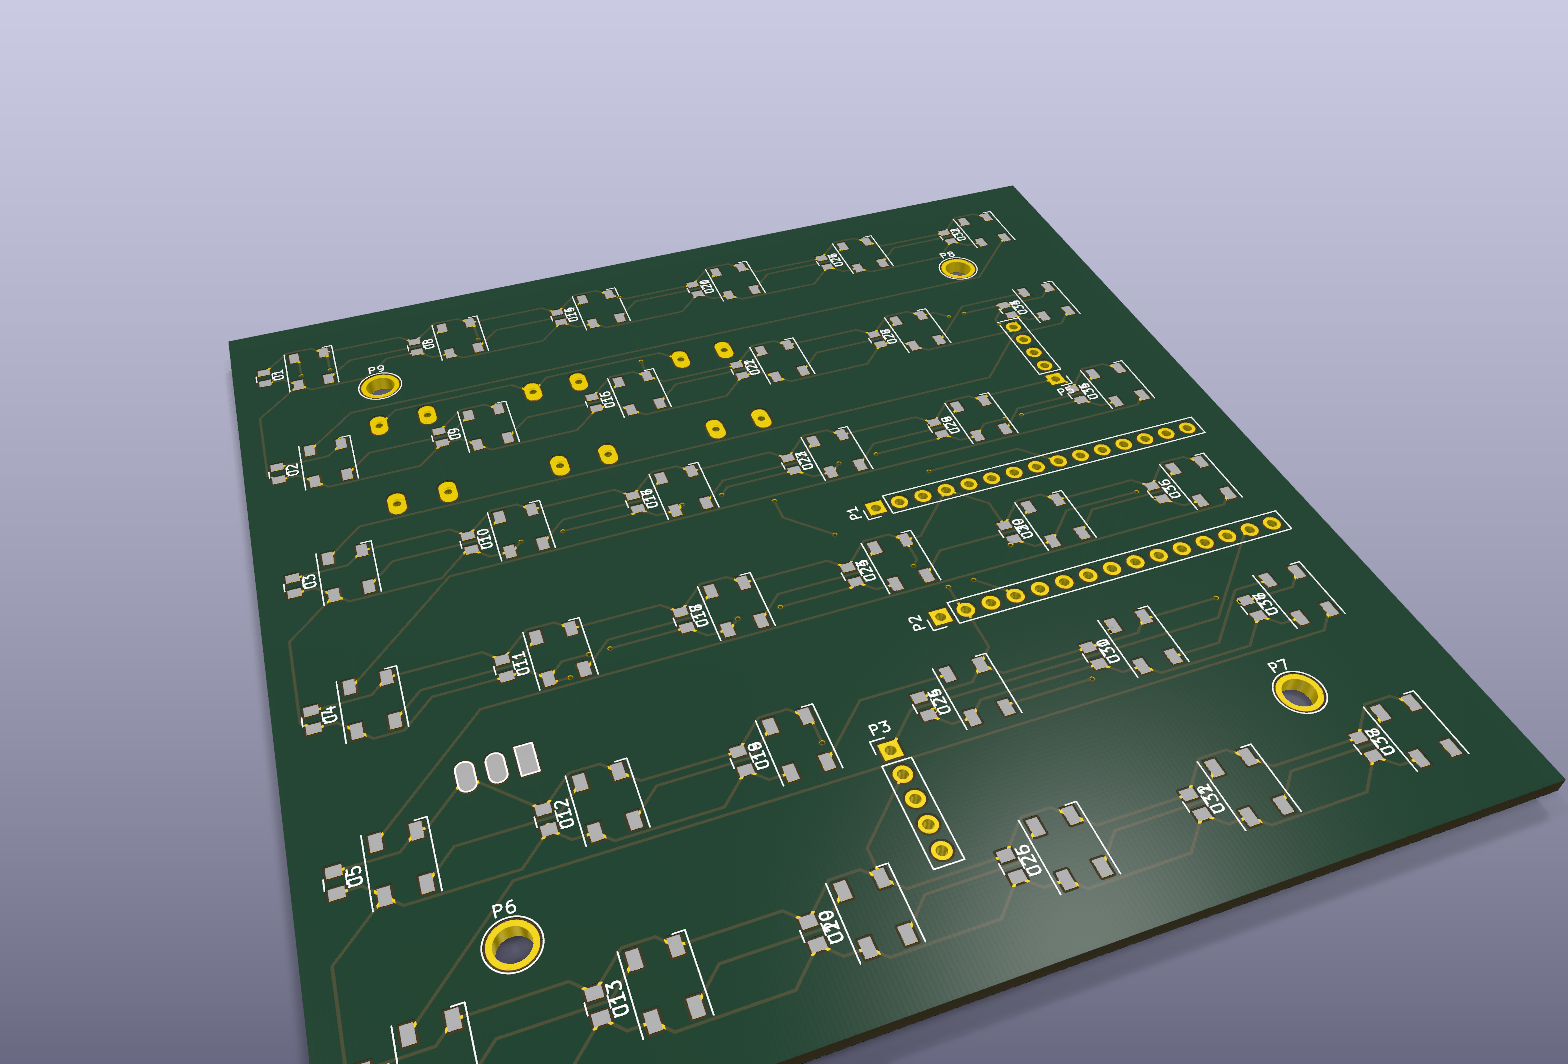
\includegraphics[width=0.78\textwidth]{hangul_3d.png}\\[2pt]
{\small Hangul-Clock (PCBench), routed by a default \texttt{tracemaker route} run: 209 of 209 connections in 44 s. KiCad 10 render.}
\end{center}

\begin{abstract}
\noindent This report follows one command, \opt{tracemaker route board.kicad_pcb -o out.kicad_pcb} with no other options, from the
command line to the written board. It is built from the code, not from the design documents: every step and every decision names
the function and line that makes it (\code{route_job.cpp}, \code{router.cpp}). The documents and the code differ in a few places,
and Section~\ref{sec:disagree} lists them. Three real boards were routed with the default settings for the figures: Hangul-Clock (two
layers, completes), the EtherCAT shield (two layers, a dense QFN, 247 of 272) and \texttt{plane\_smd} (four layers with planes, 42 of 47).
Extra runs show what the most useful options change.

\textbf{In short.} A default run is a \emph{portfolio}: eight differently tuned routers race on eight threads, each with up to
120 seconds. The one that routes the most connections wins; ties go to fewer vias, then shorter copper. If connections are still open,
a \emph{relax rescue} runs two more portfolios: one starts from the routes it has, the other from nothing. Each routes under 60\,\%
and 80\,\% of the clearance first, then pulls the copper back to the real rules. A rescue result is kept only if it routes more. Then come the repair stages,
writing the board (only new copper is added) and a proof, for every pin still open, of \emph{why} it is open. Nothing is committed to
the board without the exact geometric check. A default run is limited by wall time, not by work, so it is not repeatable across machines;
\opt{--work N} makes it so.
\end{abstract}

\tableofcontents
\newpage

%% ======================================================================
\section{The default run in one page}
\label{sec:onepage}

\begin{figure}[H]
\centering
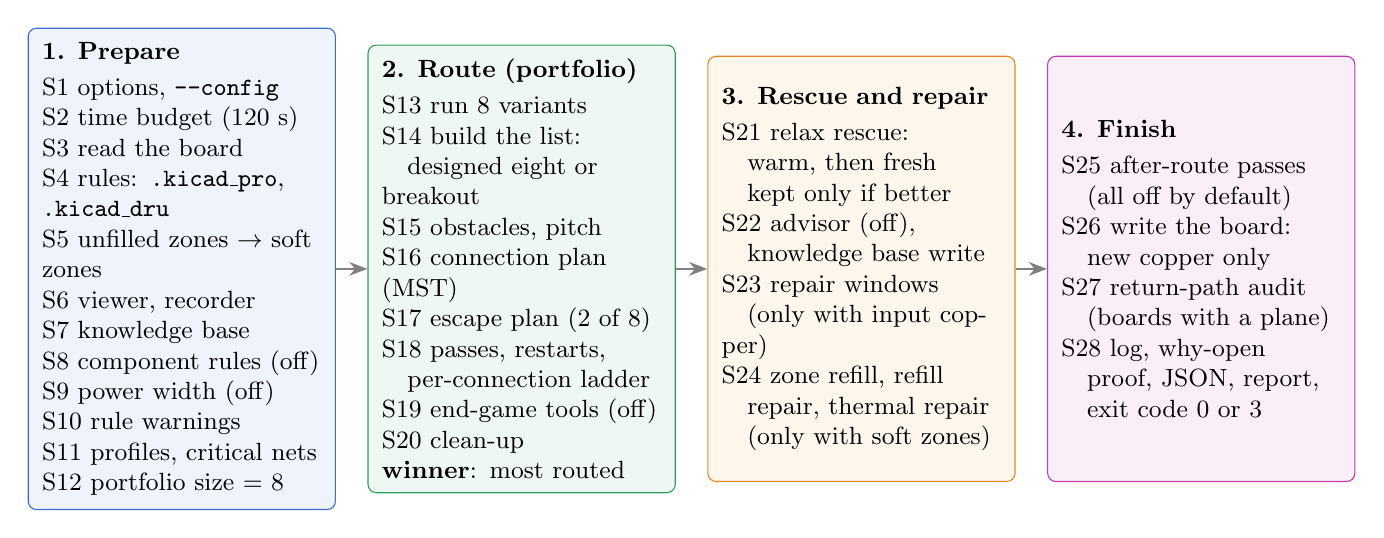
\begin{tikzpicture}[font=\small, node distance=4mm,
  ph/.style={draw=#1, fill=#1!8, rounded corners=3pt, text width=3.55cm, align=left, inner sep=5pt, minimum height=5.4cm},
  hd/.style={font=\bfseries\small, text=#1}]
\node[ph=accent] (p1) {\textbf{1. Prepare}\\[2pt]
  S1 options, \opt{--config}\\ S2 time budget (120 s)\\ S3 read the board\\ S4 rules: \texttt{.kicad\_pro}, \texttt{.kicad\_dru}\\
  S5 unfilled zones $\to$ soft zones\\ S6 viewer, recorder\\ S7 knowledge base\\ S8 component rules (off)\\ S9 power width (off)\\
  S10 rule warnings\\ S11 profiles, critical nets\\ S12 portfolio size = 8};
\node[ph=okgreen, right=of p1] (p2) {\textbf{2. Route (portfolio)}\\[2pt]
  S13 run 8 variants\\ S14 build the list:\\ \quad designed eight or breakout\\ S15 obstacles, pitch\\ S16 connection plan (MST)\\
  S17 escape plan (2 of 8)\\ S18 passes, restarts,\\ \quad per-connection ladder\\ S19 end-game tools (off)\\ S20 clean-up\\
  \textbf{winner}: most routed};
\node[ph=warn, right=of p2] (p3) {\textbf{3. Rescue and repair}\\[2pt]
  S21 relax rescue:\\ \quad warm, then fresh\\ \quad kept only if better\\ S22 advisor (off),\\ \quad knowledge base write\\
  S23 repair windows\\ \quad (only with input copper)\\ S24 zone refill, refill\\ \quad repair, thermal repair\\ \quad (only with soft zones)};
\node[ph=mag, right=of p3] (p4) {\textbf{4. Finish}\\[2pt]
  S25 after-route passes\\ \quad (all off by default)\\ S26 write the board:\\ \quad new copper only\\ S27 return-path audit\\
  \quad (boards with a plane)\\ S28 log, why-open\\ \quad proof, JSON, report,\\ \quad exit code 0 or 3};
\draw[-{Stealth}, thick, black!50] (p1) -- (p2);
\draw[-{Stealth}, thick, black!50] (p2) -- (p3);
\draw[-{Stealth}, thick, black!50] (p3) -- (p4);
\end{tikzpicture}
\caption{The 28 steps of a default run in four phases. Steps marked ``off'' are skipped unless an option asks for them; ``only
with'' steps run when the board needs them. Section~\ref{sec:walk} takes the steps one by one, Section~\ref{sec:tree} gives the decisions
as trees.}
\label{fig:pipeline}
\end{figure}

\begin{keypoint}
\textbf{What a default run decides for you}
\begin{itemize}
\item \textbf{Eight routers, not one.} The portfolio size follows \opt{--threads} (8) up to eight. The designed eight differ in bend
  model, connection order, via and crossing costs, lattice pitch, whether dense-package escapes are planned, and which end of a
  connection the search starts from (Table~\ref{tab:variants}).
\item \textbf{A wall-clock limit per stage.} \opt{--time 120} applies to the plain portfolio, and again to each rescue pass, so a
  board left open can take about three times \opt{--time} (EtherCAT: 401 s). There is no work budget unless \opt{--work} is given.
\item \textbf{Failure memory is on.} The knowledge base (\code{~/.local/share/tracemaker/kb.sqlite}) puts connections that failed on
  this board before at the front of every variant's order, and records this run's failures. A second run on the same board starts
  differently; benchmarks use \opt{--no-kb}.
\item \textbf{Existing copper is kept.} Tracks and vias already on the board, locked or not, become fixed obstacles. Only the repair
  windows (on automatically when the input had unlocked copper) can lift unlocked copper, and only to route more.
\item \textbf{Clearance is never given away.} The relax rescue routes under lower clearance, but only routes that are legal under the
  board's own rules are kept, and every commit passes the exact geometric check.
\item \textbf{Open connections are explained.} For every pin left open the run proves whether a track could leave it at all, past the fixed
  copper, and says what would help (Section~\ref{sec:whyopen}).
\end{itemize}
\end{keypoint}

\subsection{The three example runs}

\begin{table}[H]
\centering\small
\begin{tabular}{@{}lrrrrrrl@{}}
\toprule
Board & Layers & Connections & Routed & Vias & Pitch & Wall time & Kept result \\
\midrule
Hangul-Clock & 2 & 209 & \textbf{209} & 43 & 0.075 mm & 44 s & variant 2 (longest first) \\
EtherCAT shield & 2 & 272 & 247 & 141 & 0.075 mm & 401 s & fresh relax rescue \\
\texttt{plane\_smd} & 4 & 47 & 42 & 0 & 0.025 mm & 377 s & variant 5 (cheap vias) \\
\bottomrule
\end{tabular}
\caption{The default runs behind the figures: \opt{tracemaker route X.kicad_pcb -o X.routed.kicad_pcb} plus \opt{--record},
\opt{--report} and \opt{--json}, which only observe. The boards are PCBench's \texttt{unrouted.kicad\_pcb} files and TraceMaker's
own test board \texttt{tests/boards/plane\_smd}. Run on 2026-11-14 on a 56-core machine with an RTX 5060 Ti.}
\label{tab:runs}
\end{table}

%% ======================================================================
\section{The decision tree}
\label{sec:tree}

Figures~\ref{fig:tree-prep} to~\ref{fig:tree-after} are the decisions a default run takes, in the order it takes them. Each diamond is one
condition in the code; the box on the right is what happens when the branch to it is taken, and the box on the left (dotted) is what
the main flow does at that point. Thick green arrows mark what a default run on an ordinary board does. The tree has four parts:
\begin{enumerate}
\item preparing the board and rules (Figure~\ref{fig:tree-prep}),
\item building the portfolio and setting up each variant (Figure~\ref{fig:tree-portfolio}),
\item routing one connection, and the passes and restarts around it (Figure~\ref{fig:tree-connection}),
\item what happens after the portfolio (Figure~\ref{fig:tree-after}).
\end{enumerate}

\begin{figure}[p]
\centering
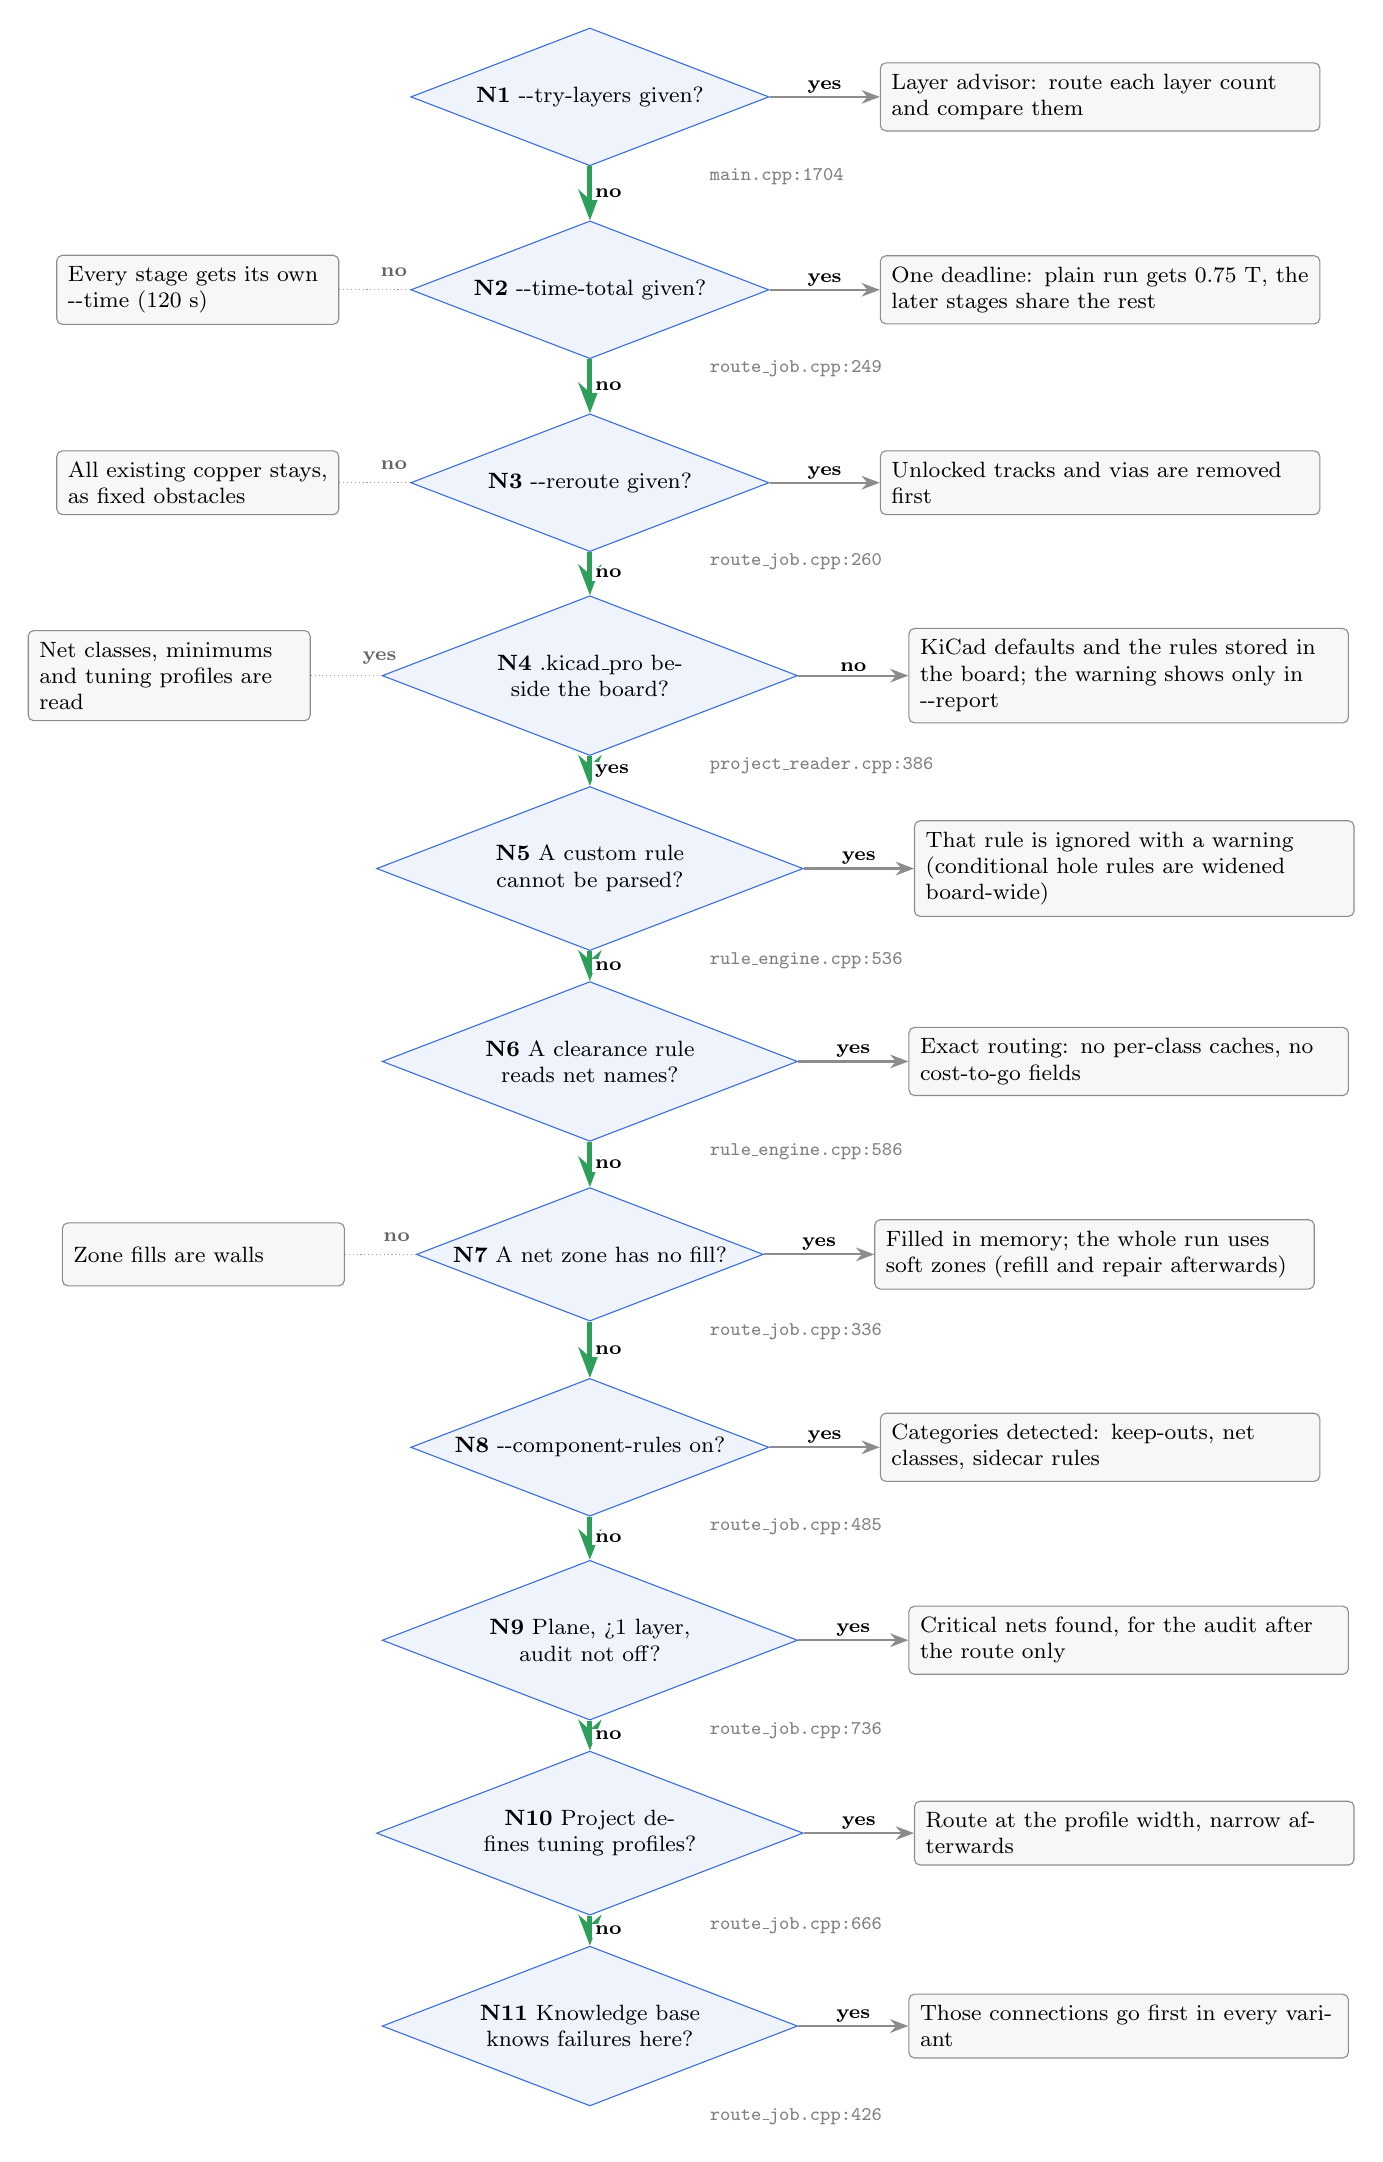
\begin{tikzpicture}[font=\footnotesize, node distance=1cm, dec/.style={draw=accent, fill=accent!8, diamond, aspect=2.6, text width=3.9cm, align=center, inner sep=0pt}, act/.style={draw=black!45, fill=black!3, rounded corners=2pt, text width=5.3cm, align=left, inner sep=4pt, minimum height=8mm}, ref/.style={font=\scriptsize\ttfamily, text=black!50}, arr/.style={-{Stealth}, draw=black!45, thick}, def/.style={-{Stealth}, draw=okgreen, line width=1.8pt}, lab/.style={font=\scriptsize\bfseries, fill=white, inner sep=1pt}]
\node[dec] (n0) at (0,0.00) {\textbf{N1} -{}-try-layers given?};
\node[act, right=1.4cm of n0] (s0) {Layer advisor: route each layer count and compare them};
\draw[arr] (n0) -- node[lab, above] {yes} (s0);
\node[ref, below right=-1mm and 1.4cm of n0.south, anchor=north west] {main.cpp:1704};
\node[dec] (n1) at (0,-2.45) {\textbf{N2} -{}-time-total given?};
\node[act, right=1.4cm of n1] (s1) {One deadline: plain run gets 0.75 T, the later stages share the rest};
\draw[arr] (n1) -- node[lab, above] {yes} (s1);
\node[act, left=0.9cm of n1, text width=3.3cm] (d1) {Every stage gets its own -{}-time (120 s)};
\draw[densely dotted, black!40] (n1) -- (d1);
\node[lab, text=black!60] at ($(n1)!0.5!(d1)+(0,0.22)$) {no};
\node[ref, below right=-1mm and 1.4cm of n1.south, anchor=north west] {route\_job.cpp:249};
\draw[def] (n0) -- node[lab, right] {no} (n1);
\node[dec] (n2) at (0,-4.90) {\textbf{N3} -{}-reroute given?};
\node[act, right=1.4cm of n2] (s2) {Unlocked tracks and vias are removed first};
\draw[arr] (n2) -- node[lab, above] {yes} (s2);
\node[act, left=0.9cm of n2, text width=3.3cm] (d2) {All existing copper stays, as fixed obstacles};
\draw[densely dotted, black!40] (n2) -- (d2);
\node[lab, text=black!60] at ($(n2)!0.5!(d2)+(0,0.22)$) {no};
\node[ref, below right=-1mm and 1.4cm of n2.south, anchor=north west] {route\_job.cpp:260};
\draw[def] (n1) -- node[lab, right] {no} (n2);
\node[dec] (n3) at (0,-7.35) {\textbf{N4} .kicad\_pro beside the board?};
\node[act, right=1.4cm of n3] (s3) {KiCad defaults and the rules stored in the board; the warning shows only in -{}-report};
\draw[arr] (n3) -- node[lab, above] {no} (s3);
\node[act, left=0.9cm of n3, text width=3.3cm] (d3) {Net classes, minimums and tuning profiles are read};
\draw[densely dotted, black!40] (n3) -- (d3);
\node[lab, text=black!60] at ($(n3)!0.5!(d3)+(0,0.22)$) {yes};
\node[ref, below right=-1mm and 1.4cm of n3.south, anchor=north west] {project\_reader.cpp:386};
\draw[def] (n2) -- node[lab, right] {no} (n3);
\node[dec] (n4) at (0,-9.80) {\textbf{N5} A custom rule cannot be parsed?};
\node[act, right=1.4cm of n4] (s4) {That rule is ignored with a warning (conditional hole rules are widened board-wide)};
\draw[arr] (n4) -- node[lab, above] {yes} (s4);
\node[ref, below right=-1mm and 1.4cm of n4.south, anchor=north west] {rule\_engine.cpp:536};
\draw[def] (n3) -- node[lab, right] {yes} (n4);
\node[dec] (n5) at (0,-12.25) {\textbf{N6} A clearance rule reads net names?};
\node[act, right=1.4cm of n5] (s5) {Exact routing: no per-class caches, no cost-to-go fields};
\draw[arr] (n5) -- node[lab, above] {yes} (s5);
\node[ref, below right=-1mm and 1.4cm of n5.south, anchor=north west] {rule\_engine.cpp:586};
\draw[def] (n4) -- node[lab, right] {no} (n5);
\node[dec] (n6) at (0,-14.70) {\textbf{N7} A net zone has no fill?};
\node[act, right=1.4cm of n6] (s6) {Filled in memory; the whole run uses soft zones (refill and repair afterwards)};
\draw[arr] (n6) -- node[lab, above] {yes} (s6);
\node[act, left=0.9cm of n6, text width=3.3cm] (d6) {Zone fills are walls};
\draw[densely dotted, black!40] (n6) -- (d6);
\node[lab, text=black!60] at ($(n6)!0.5!(d6)+(0,0.22)$) {no};
\node[ref, below right=-1mm and 1.4cm of n6.south, anchor=north west] {route\_job.cpp:336};
\draw[def] (n5) -- node[lab, right] {no} (n6);
\node[dec] (n7) at (0,-17.15) {\textbf{N8} -{}-component-rules on?};
\node[act, right=1.4cm of n7] (s7) {Categories detected: keep-outs, net classes, sidecar rules};
\draw[arr] (n7) -- node[lab, above] {yes} (s7);
\node[ref, below right=-1mm and 1.4cm of n7.south, anchor=north west] {route\_job.cpp:485};
\draw[def] (n6) -- node[lab, right] {no} (n7);
\node[dec] (n8) at (0,-19.60) {\textbf{N9} Plane, >1 layer, audit not off?};
\node[act, right=1.4cm of n8] (s8) {Critical nets found, for the audit after the route only};
\draw[arr] (n8) -- node[lab, above] {yes} (s8);
\node[ref, below right=-1mm and 1.4cm of n8.south, anchor=north west] {route\_job.cpp:736};
\draw[def] (n7) -- node[lab, right] {no} (n8);
\node[dec] (n9) at (0,-22.05) {\textbf{N10} Project defines tuning profiles?};
\node[act, right=1.4cm of n9] (s9) {Route at the profile width, narrow afterwards};
\draw[arr] (n9) -- node[lab, above] {yes} (s9);
\node[ref, below right=-1mm and 1.4cm of n9.south, anchor=north west] {route\_job.cpp:666};
\draw[def] (n8) -- node[lab, right] {no} (n9);
\node[dec] (n10) at (0,-24.50) {\textbf{N11} Knowledge base knows failures here?};
\node[act, right=1.4cm of n10] (s10) {Those connections go first in every variant};
\draw[arr] (n10) -- node[lab, above] {yes} (s10);
\node[ref, below right=-1mm and 1.4cm of n10.south, anchor=north west] {route\_job.cpp:426};
\draw[def] (n9) -- node[lab, right] {no} (n10);
\end{tikzpicture}
\caption{Before routing: reading the board and the rules (steps S1--S12). Green arrows: the branch a default run takes on an ordinary two-layer board with a project file, filled zones and a GPU. The grey reference is the line of the decision in the code.}
\label{fig:tree-prep}
\end{figure}

\begin{figure}[p]
\centering
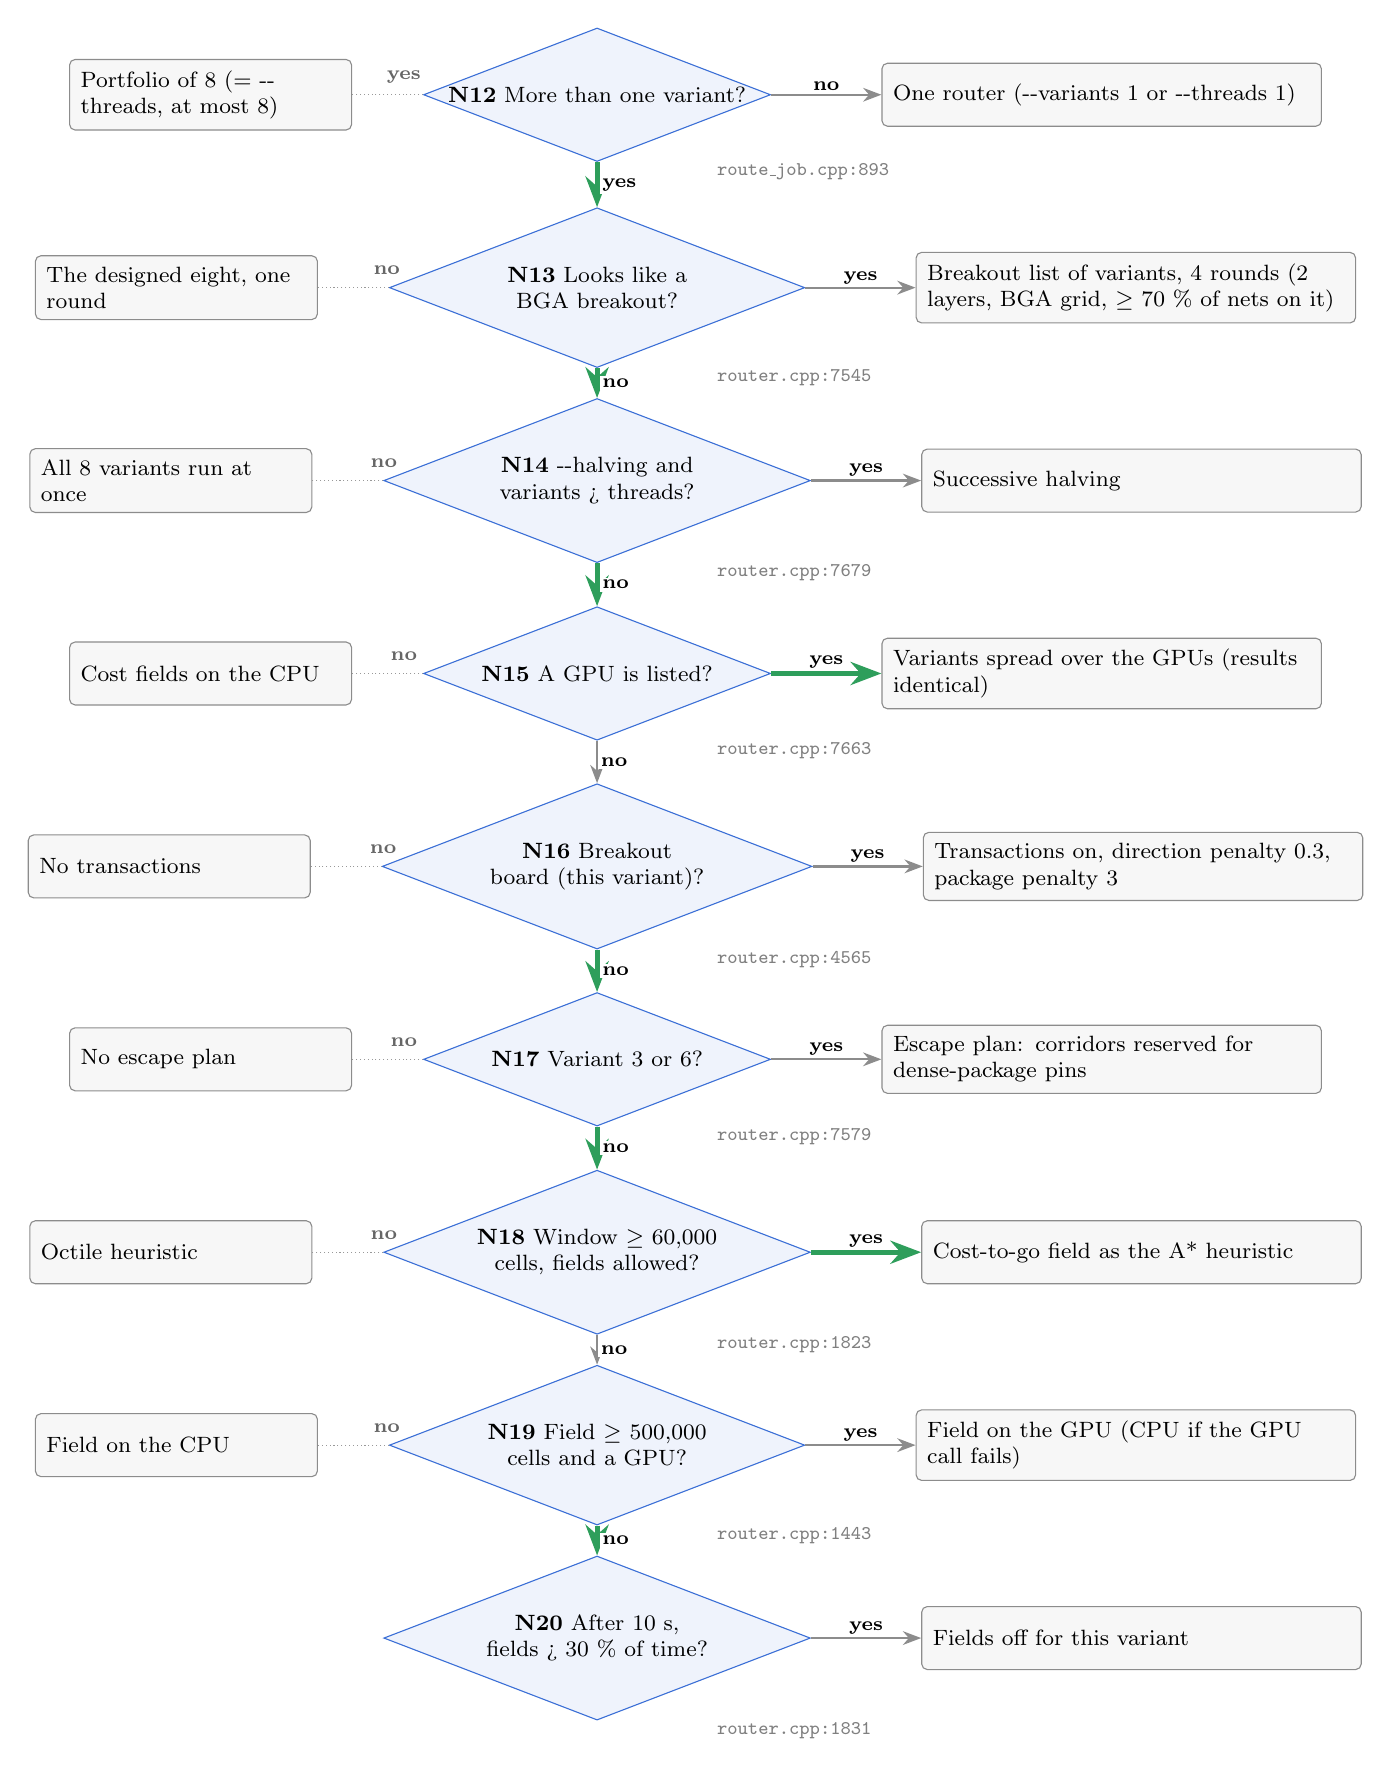
\begin{tikzpicture}[font=\footnotesize, node distance=1cm, dec/.style={draw=accent, fill=accent!8, diamond, aspect=2.6, text width=3.9cm, align=center, inner sep=0pt}, act/.style={draw=black!45, fill=black!3, rounded corners=2pt, text width=5.3cm, align=left, inner sep=4pt, minimum height=8mm}, ref/.style={font=\scriptsize\ttfamily, text=black!50}, arr/.style={-{Stealth}, draw=black!45, thick}, def/.style={-{Stealth}, draw=okgreen, line width=1.8pt}, lab/.style={font=\scriptsize\bfseries, fill=white, inner sep=1pt}]
\node[dec] (n0) at (0,0.00) {\textbf{N12} More than one variant?};
\node[act, right=1.4cm of n0] (s0) {One router (-{}-variants 1 or -{}-threads 1)};
\draw[arr] (n0) -- node[lab, above] {no} (s0);
\node[act, left=0.9cm of n0, text width=3.3cm] (d0) {Portfolio of 8 (= -{}-threads, at most 8)};
\draw[densely dotted, black!40] (n0) -- (d0);
\node[lab, text=black!60] at ($(n0)!0.5!(d0)+(0,0.22)$) {yes};
\node[ref, below right=-1mm and 1.4cm of n0.south, anchor=north west] {route\_job.cpp:893};
\node[dec] (n1) at (0,-2.45) {\textbf{N13} Looks like a BGA breakout?};
\node[act, right=1.4cm of n1] (s1) {Breakout list of variants, 4 rounds (2 layers, BGA grid, $\geq$ 70 \% of nets on it)};
\draw[arr] (n1) -- node[lab, above] {yes} (s1);
\node[act, left=0.9cm of n1, text width=3.3cm] (d1) {The designed eight, one round};
\draw[densely dotted, black!40] (n1) -- (d1);
\node[lab, text=black!60] at ($(n1)!0.5!(d1)+(0,0.22)$) {no};
\node[ref, below right=-1mm and 1.4cm of n1.south, anchor=north west] {router.cpp:7545};
\draw[def] (n0) -- node[lab, right] {yes} (n1);
\node[dec] (n2) at (0,-4.90) {\textbf{N14} -{}-halving and variants > threads?};
\node[act, right=1.4cm of n2] (s2) {Successive halving};
\draw[arr] (n2) -- node[lab, above] {yes} (s2);
\node[act, left=0.9cm of n2, text width=3.3cm] (d2) {All 8 variants run at once};
\draw[densely dotted, black!40] (n2) -- (d2);
\node[lab, text=black!60] at ($(n2)!0.5!(d2)+(0,0.22)$) {no};
\node[ref, below right=-1mm and 1.4cm of n2.south, anchor=north west] {router.cpp:7679};
\draw[def] (n1) -- node[lab, right] {no} (n2);
\node[dec] (n3) at (0,-7.35) {\textbf{N15} A GPU is listed?};
\node[act, right=1.4cm of n3] (s3) {Variants spread over the GPUs (results identical)};
\draw[def] (n3) -- node[lab, above] {yes} (s3);
\node[act, left=0.9cm of n3, text width=3.3cm] (d3) {Cost fields on the CPU};
\draw[densely dotted, black!40] (n3) -- (d3);
\node[lab, text=black!60] at ($(n3)!0.5!(d3)+(0,0.22)$) {no};
\node[ref, below right=-1mm and 1.4cm of n3.south, anchor=north west] {router.cpp:7663};
\draw[def] (n2) -- node[lab, right] {no} (n3);
\node[dec] (n4) at (0,-9.80) {\textbf{N16} Breakout board (this variant)?};
\node[act, right=1.4cm of n4] (s4) {Transactions on, direction penalty 0.3, package penalty 3};
\draw[arr] (n4) -- node[lab, above] {yes} (s4);
\node[act, left=0.9cm of n4, text width=3.3cm] (d4) {No transactions};
\draw[densely dotted, black!40] (n4) -- (d4);
\node[lab, text=black!60] at ($(n4)!0.5!(d4)+(0,0.22)$) {no};
\node[ref, below right=-1mm and 1.4cm of n4.south, anchor=north west] {router.cpp:4565};
\draw[arr] (n3) -- node[lab, right] {no} (n4);
\node[dec] (n5) at (0,-12.25) {\textbf{N17} Variant 3 or 6?};
\node[act, right=1.4cm of n5] (s5) {Escape plan: corridors reserved for dense-package pins};
\draw[arr] (n5) -- node[lab, above] {yes} (s5);
\node[act, left=0.9cm of n5, text width=3.3cm] (d5) {No escape plan};
\draw[densely dotted, black!40] (n5) -- (d5);
\node[lab, text=black!60] at ($(n5)!0.5!(d5)+(0,0.22)$) {no};
\node[ref, below right=-1mm and 1.4cm of n5.south, anchor=north west] {router.cpp:7579};
\draw[def] (n4) -- node[lab, right] {no} (n5);
\node[dec] (n6) at (0,-14.70) {\textbf{N18} Window $\geq$ 60,000 cells, fields allowed?};
\node[act, right=1.4cm of n6] (s6) {Cost-to-go field as the A* heuristic};
\draw[def] (n6) -- node[lab, above] {yes} (s6);
\node[act, left=0.9cm of n6, text width=3.3cm] (d6) {Octile heuristic};
\draw[densely dotted, black!40] (n6) -- (d6);
\node[lab, text=black!60] at ($(n6)!0.5!(d6)+(0,0.22)$) {no};
\node[ref, below right=-1mm and 1.4cm of n6.south, anchor=north west] {router.cpp:1823};
\draw[def] (n5) -- node[lab, right] {no} (n6);
\node[dec] (n7) at (0,-17.15) {\textbf{N19} Field $\geq$ 500,000 cells and a GPU?};
\node[act, right=1.4cm of n7] (s7) {Field on the GPU (CPU if the GPU call fails)};
\draw[arr] (n7) -- node[lab, above] {yes} (s7);
\node[act, left=0.9cm of n7, text width=3.3cm] (d7) {Field on the CPU};
\draw[densely dotted, black!40] (n7) -- (d7);
\node[lab, text=black!60] at ($(n7)!0.5!(d7)+(0,0.22)$) {no};
\node[ref, below right=-1mm and 1.4cm of n7.south, anchor=north west] {router.cpp:1443};
\draw[arr] (n6) -- node[lab, right] {no} (n7);
\node[dec] (n8) at (0,-19.60) {\textbf{N20} After 10 s, fields > 30 \% of time?};
\node[act, right=1.4cm of n8] (s8) {Fields off for this variant};
\draw[arr] (n8) -- node[lab, above] {yes} (s8);
\node[ref, below right=-1mm and 1.4cm of n8.south, anchor=north west] {router.cpp:1831};
\draw[def] (n7) -- node[lab, right] {no} (n8);
\end{tikzpicture}
\caption{The portfolio and one variant's set-up (steps S13--S17). Green arrows: the branch a default run takes on an ordinary two-layer board with a project file, filled zones and a GPU. The grey reference is the line of the decision in the code.}
\label{fig:tree-portfolio}
\end{figure}

\begin{figure}[p]
\centering
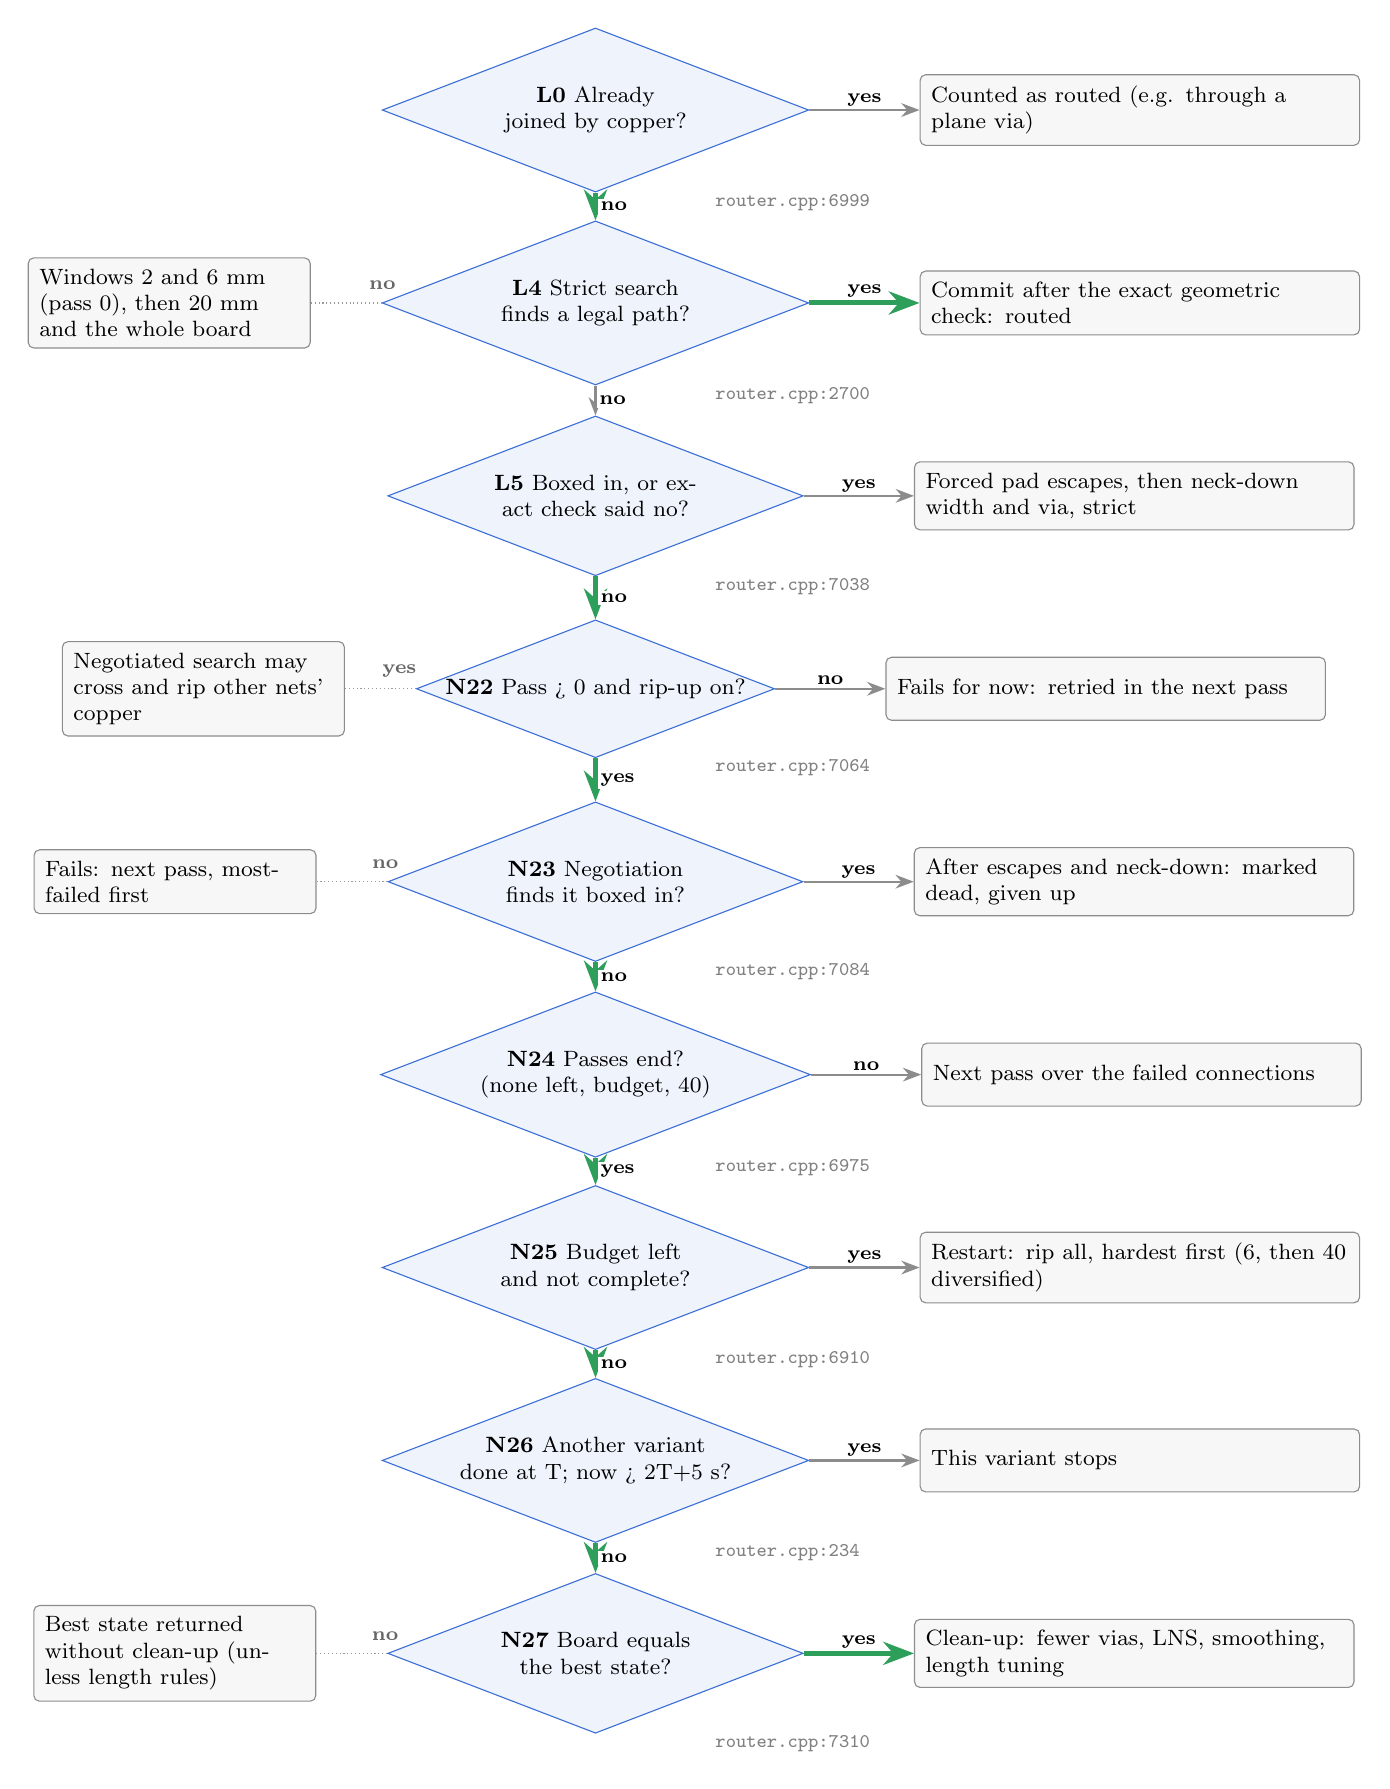
\begin{tikzpicture}[font=\footnotesize, node distance=1cm, dec/.style={draw=accent, fill=accent!8, diamond, aspect=2.6, text width=3.9cm, align=center, inner sep=0pt}, act/.style={draw=black!45, fill=black!3, rounded corners=2pt, text width=5.3cm, align=left, inner sep=4pt, minimum height=8mm}, ref/.style={font=\scriptsize\ttfamily, text=black!50}, arr/.style={-{Stealth}, draw=black!45, thick}, def/.style={-{Stealth}, draw=okgreen, line width=1.8pt}, lab/.style={font=\scriptsize\bfseries, fill=white, inner sep=1pt}]
\node[dec] (n0) at (0,0.00) {\textbf{L0} Already joined by copper?};
\node[act, right=1.4cm of n0] (s0) {Counted as routed (e.g. through a plane via)};
\draw[arr] (n0) -- node[lab, above] {yes} (s0);
\node[ref, below right=-1mm and 1.4cm of n0.south, anchor=north west] {router.cpp:6999};
\node[dec] (n1) at (0,-2.45) {\textbf{L4} Strict search finds a legal path?};
\node[act, right=1.4cm of n1] (s1) {Commit after the exact geometric check: routed};
\draw[def] (n1) -- node[lab, above] {yes} (s1);
\node[act, left=0.9cm of n1, text width=3.3cm] (d1) {Windows 2 and 6 mm (pass 0), then 20 mm and the whole board};
\draw[densely dotted, black!40] (n1) -- (d1);
\node[lab, text=black!60] at ($(n1)!0.5!(d1)+(0,0.22)$) {no};
\node[ref, below right=-1mm and 1.4cm of n1.south, anchor=north west] {router.cpp:2700};
\draw[def] (n0) -- node[lab, right] {no} (n1);
\node[dec] (n2) at (0,-4.90) {\textbf{L5} Boxed in, or exact check said no?};
\node[act, right=1.4cm of n2] (s2) {Forced pad escapes, then neck-down width and via, strict};
\draw[arr] (n2) -- node[lab, above] {yes} (s2);
\node[ref, below right=-1mm and 1.4cm of n2.south, anchor=north west] {router.cpp:7038};
\draw[arr] (n1) -- node[lab, right] {no} (n2);
\node[dec] (n3) at (0,-7.35) {\textbf{N22} Pass > 0 and rip-up on?};
\node[act, right=1.4cm of n3] (s3) {Fails for now: retried in the next pass};
\draw[arr] (n3) -- node[lab, above] {no} (s3);
\node[act, left=0.9cm of n3, text width=3.3cm] (d3) {Negotiated search may cross and rip other nets' copper};
\draw[densely dotted, black!40] (n3) -- (d3);
\node[lab, text=black!60] at ($(n3)!0.5!(d3)+(0,0.22)$) {yes};
\node[ref, below right=-1mm and 1.4cm of n3.south, anchor=north west] {router.cpp:7064};
\draw[def] (n2) -- node[lab, right] {no} (n3);
\node[dec] (n4) at (0,-9.80) {\textbf{N23} Negotiation finds it boxed in?};
\node[act, right=1.4cm of n4] (s4) {After escapes and neck-down: marked dead, given up};
\draw[arr] (n4) -- node[lab, above] {yes} (s4);
\node[act, left=0.9cm of n4, text width=3.3cm] (d4) {Fails: next pass, most-failed first};
\draw[densely dotted, black!40] (n4) -- (d4);
\node[lab, text=black!60] at ($(n4)!0.5!(d4)+(0,0.22)$) {no};
\node[ref, below right=-1mm and 1.4cm of n4.south, anchor=north west] {router.cpp:7084};
\draw[def] (n3) -- node[lab, right] {yes} (n4);
\node[dec] (n5) at (0,-12.25) {\textbf{N24} Passes end? (none left, budget, 40)};
\node[act, right=1.4cm of n5] (s5) {Next pass over the failed connections};
\draw[arr] (n5) -- node[lab, above] {no} (s5);
\node[ref, below right=-1mm and 1.4cm of n5.south, anchor=north west] {router.cpp:6975};
\draw[def] (n4) -- node[lab, right] {no} (n5);
\node[dec] (n6) at (0,-14.70) {\textbf{N25} Budget left and not complete?};
\node[act, right=1.4cm of n6] (s6) {Restart: rip all, hardest first (6, then 40 diversified)};
\draw[arr] (n6) -- node[lab, above] {yes} (s6);
\node[ref, below right=-1mm and 1.4cm of n6.south, anchor=north west] {router.cpp:6910};
\draw[def] (n5) -- node[lab, right] {yes} (n6);
\node[dec] (n7) at (0,-17.15) {\textbf{N26} Another variant done at T; now > 2T+5 s?};
\node[act, right=1.4cm of n7] (s7) {This variant stops};
\draw[arr] (n7) -- node[lab, above] {yes} (s7);
\node[ref, below right=-1mm and 1.4cm of n7.south, anchor=north west] {router.cpp:234};
\draw[def] (n6) -- node[lab, right] {no} (n7);
\node[dec] (n8) at (0,-19.60) {\textbf{N27} Board equals the best state?};
\node[act, right=1.4cm of n8] (s8) {Clean-up: fewer vias, LNS, smoothing, length tuning};
\draw[def] (n8) -- node[lab, above] {yes} (s8);
\node[act, left=0.9cm of n8, text width=3.3cm] (d8) {Best state returned without clean-up (unless length rules)};
\draw[densely dotted, black!40] (n8) -- (d8);
\node[lab, text=black!60] at ($(n8)!0.5!(d8)+(0,0.22)$) {no};
\node[ref, below right=-1mm and 1.4cm of n8.south, anchor=north west] {router.cpp:7310};
\draw[def] (n7) -- node[lab, right] {no} (n8);
\end{tikzpicture}
\caption{One connection inside a variant, and the passes and restarts (steps S18--S20). Green arrows: the branch a default run takes on an ordinary two-layer board with a project file, filled zones and a GPU. The grey reference is the line of the decision in the code.}
\label{fig:tree-connection}
\end{figure}

\begin{figure}[p]
\centering
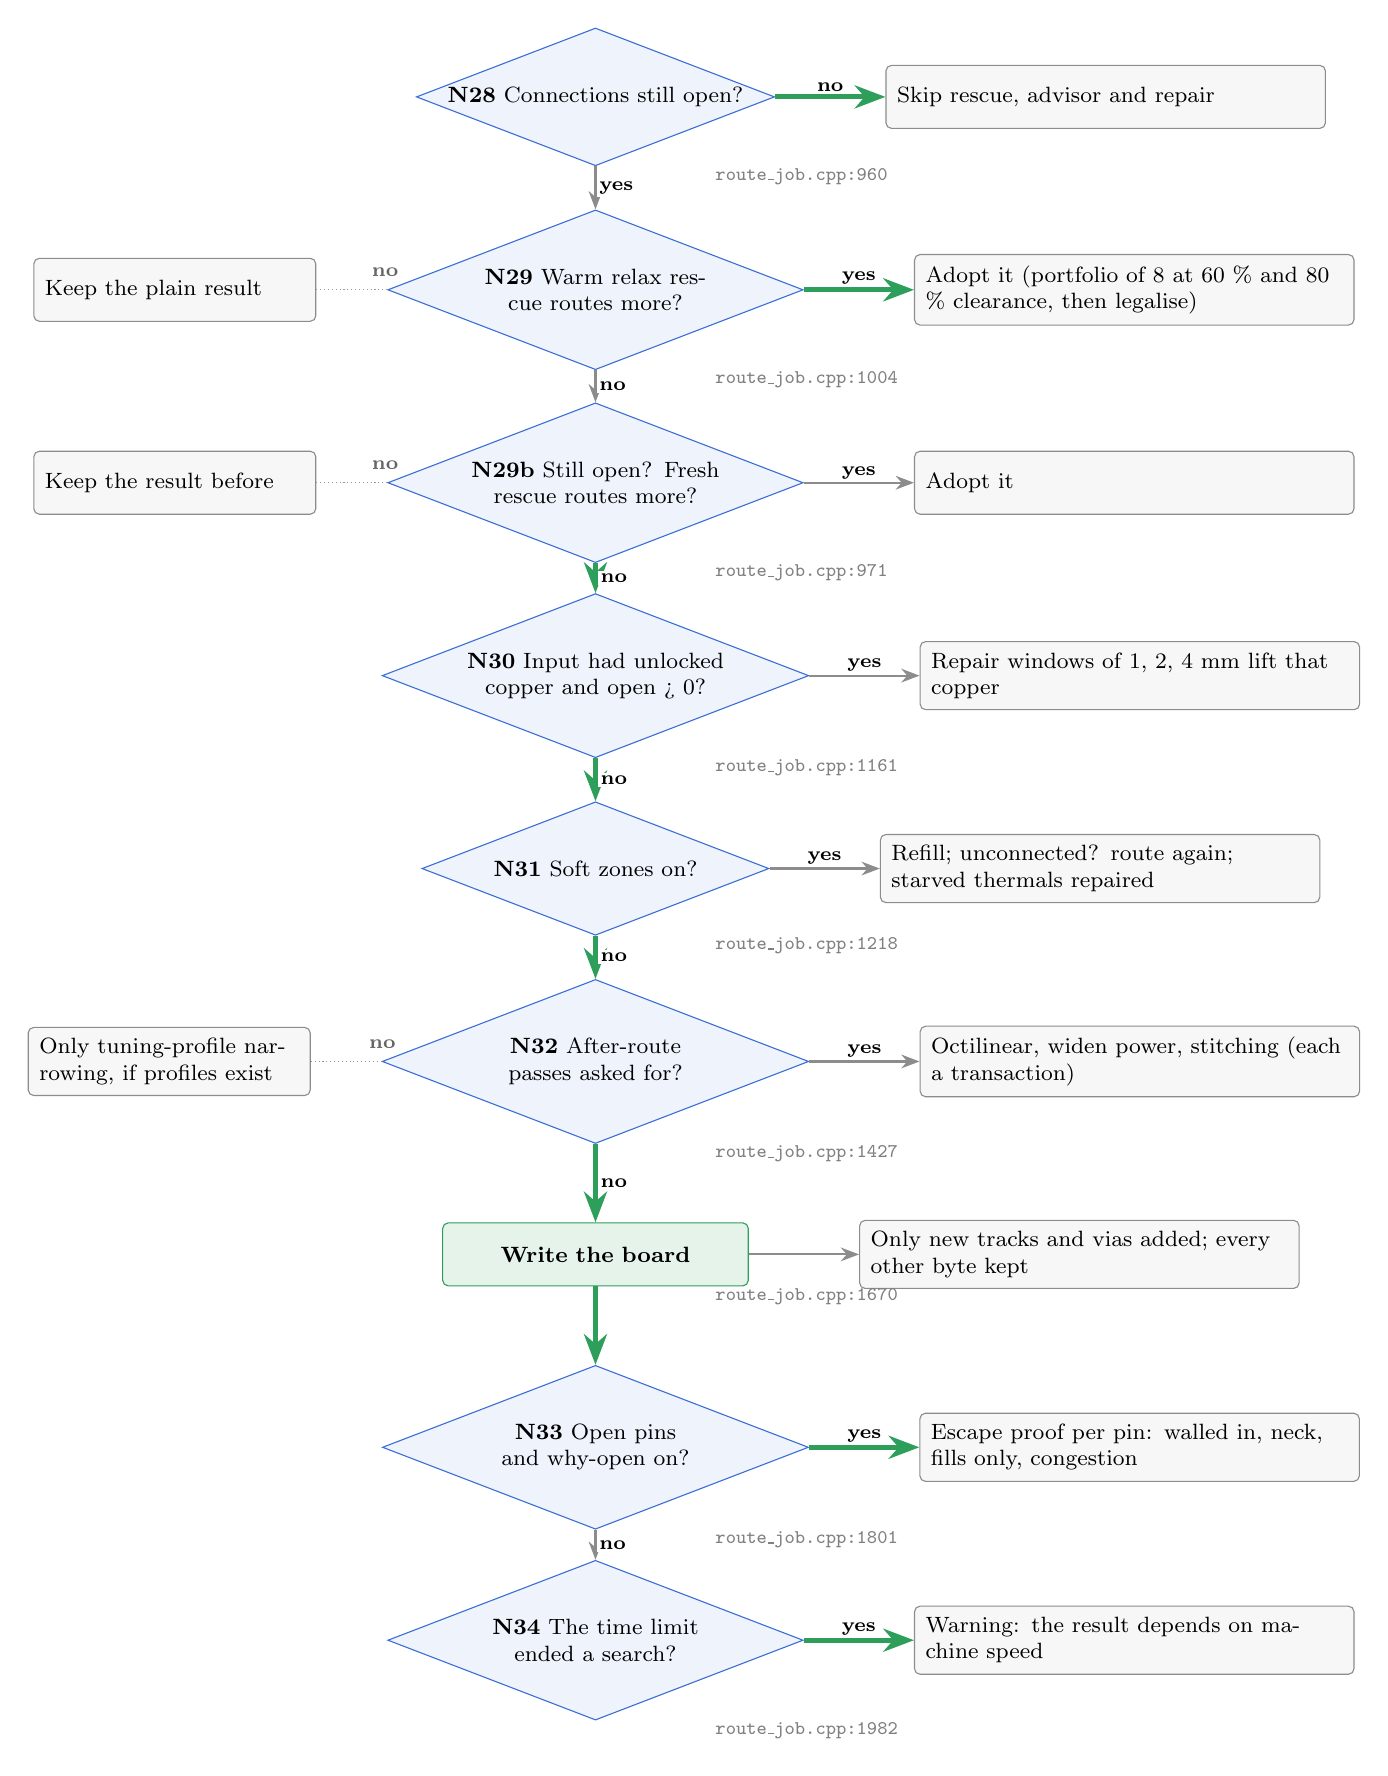
\begin{tikzpicture}[font=\footnotesize, node distance=1cm, dec/.style={draw=accent, fill=accent!8, diamond, aspect=2.6, text width=3.9cm, align=center, inner sep=0pt}, act/.style={draw=black!45, fill=black!3, rounded corners=2pt, text width=5.3cm, align=left, inner sep=4pt, minimum height=8mm}, ref/.style={font=\scriptsize\ttfamily, text=black!50}, arr/.style={-{Stealth}, draw=black!45, thick}, def/.style={-{Stealth}, draw=okgreen, line width=1.8pt}, lab/.style={font=\scriptsize\bfseries, fill=white, inner sep=1pt}]
\node[dec] (n0) at (0,0.00) {\textbf{N28} Connections still open?};
\node[act, right=1.4cm of n0] (s0) {Skip rescue, advisor and repair};
\draw[def] (n0) -- node[lab, above] {no} (s0);
\node[ref, below right=-1mm and 1.4cm of n0.south, anchor=north west] {route\_job.cpp:960};
\node[dec] (n1) at (0,-2.45) {\textbf{N29} Warm relax rescue routes more?};
\node[act, right=1.4cm of n1] (s1) {Adopt it (portfolio of 8 at 60 \% and 80 \% clearance, then legalise)};
\draw[def] (n1) -- node[lab, above] {yes} (s1);
\node[act, left=0.9cm of n1, text width=3.3cm] (d1) {Keep the plain result};
\draw[densely dotted, black!40] (n1) -- (d1);
\node[lab, text=black!60] at ($(n1)!0.5!(d1)+(0,0.22)$) {no};
\node[ref, below right=-1mm and 1.4cm of n1.south, anchor=north west] {route\_job.cpp:1004};
\draw[arr] (n0) -- node[lab, right] {yes} (n1);
\node[dec] (n2) at (0,-4.90) {\textbf{N29b} Still open? Fresh rescue routes more?};
\node[act, right=1.4cm of n2] (s2) {Adopt it};
\draw[arr] (n2) -- node[lab, above] {yes} (s2);
\node[act, left=0.9cm of n2, text width=3.3cm] (d2) {Keep the result before};
\draw[densely dotted, black!40] (n2) -- (d2);
\node[lab, text=black!60] at ($(n2)!0.5!(d2)+(0,0.22)$) {no};
\node[ref, below right=-1mm and 1.4cm of n2.south, anchor=north west] {route\_job.cpp:971};
\draw[arr] (n1) -- node[lab, right] {no} (n2);
\node[dec] (n3) at (0,-7.35) {\textbf{N30} Input had unlocked copper and open > 0?};
\node[act, right=1.4cm of n3] (s3) {Repair windows of 1, 2, 4 mm lift that copper};
\draw[arr] (n3) -- node[lab, above] {yes} (s3);
\node[ref, below right=-1mm and 1.4cm of n3.south, anchor=north west] {route\_job.cpp:1161};
\draw[def] (n2) -- node[lab, right] {no} (n3);
\node[dec] (n4) at (0,-9.80) {\textbf{N31} Soft zones on?};
\node[act, right=1.4cm of n4] (s4) {Refill; unconnected? route again; starved thermals repaired};
\draw[arr] (n4) -- node[lab, above] {yes} (s4);
\node[ref, below right=-1mm and 1.4cm of n4.south, anchor=north west] {route\_job.cpp:1218};
\draw[def] (n3) -- node[lab, right] {no} (n4);
\node[dec] (n5) at (0,-12.25) {\textbf{N32} After-route passes asked for?};
\node[act, right=1.4cm of n5] (s5) {Octilinear, widen power, stitching (each a transaction)};
\draw[arr] (n5) -- node[lab, above] {yes} (s5);
\node[act, left=0.9cm of n5, text width=3.3cm] (d5) {Only tuning-profile narrowing, if profiles exist};
\draw[densely dotted, black!40] (n5) -- (d5);
\node[lab, text=black!60] at ($(n5)!0.5!(d5)+(0,0.22)$) {no};
\node[ref, below right=-1mm and 1.4cm of n5.south, anchor=north west] {route\_job.cpp:1427};
\draw[def] (n4) -- node[lab, right] {no} (n5);
\node[act, fill=okgreen!12, draw=okgreen, text width=3.6cm, align=center] (n6) at (0,-14.70) {\textbf{Write the board}};
\node[act, right=1.4cm of n6] (s6) {Only new tracks and vias added; every other byte kept};
\draw[arr] (n6) -- (s6);
\node[ref, below right=-1mm and 1.4cm of n6.south, anchor=north west] {route\_job.cpp:1670};
\draw[def] (n5) -- node[lab, right] {no} (n6);
\node[dec] (n7) at (0,-17.15) {\textbf{N33} Open pins and why-open on?};
\node[act, right=1.4cm of n7] (s7) {Escape proof per pin: walled in, neck, fills only, congestion};
\draw[def] (n7) -- node[lab, above] {yes} (s7);
\node[ref, below right=-1mm and 1.4cm of n7.south, anchor=north west] {route\_job.cpp:1801};
\draw[def] (n6) -- node[lab, right] {} (n7);
\node[dec] (n8) at (0,-19.60) {\textbf{N34} The time limit ended a search?};
\node[act, right=1.4cm of n8] (s8) {Warning: the result depends on machine speed};
\draw[def] (n8) -- node[lab, above] {yes} (s8);
\node[ref, below right=-1mm and 1.4cm of n8.south, anchor=north west] {route\_job.cpp:1982};
\draw[arr] (n7) -- node[lab, right] {no} (n8);
\end{tikzpicture}
\caption{After the portfolio: rescue, repair, refill, write and explain (steps S21--S28). Green arrows: the branch a default run takes on an ordinary two-layer board with a project file, filled zones and a GPU. The grey reference is the line of the decision in the code.}
\label{fig:tree-after}
\end{figure}


%% ======================================================================
\section{The pipeline, step by step}
\label{sec:walk}

\subsection{Preparing: options, time and the board (S1--S3)}

\step{S1 Options.} The \texttt{route} subcommand fills two structures: \code{RouterOptions} (everything one router needs) and
\code{RouteJob} (the stages around the routers). A \opt{--config FILE} of \texttt{name = value} lines, as \texttt{tracemaker tui} saves
them, is read first; the command line wins. Every option given is recorded for the report, so a run report says how it was made.

\step{S2 Time.} Without \opt{--time-total}, the plain run gets \opt{--time} (120 s), and so does each later stage that routes: each
rescue pass, each advisor round, the refill repair. With \opt{--time-total T} there is one deadline: the plain run gets
$0.75\,T$ (\opt{--rescue-share}) when a rescue may follow, and the later stages share what is left (D186).

\step{S3 The board.} The \texttt{.kicad\_pcb} is parsed into an s-expression document and a board model. All existing tracks and vias,
locked or not, become \emph{fixed copper}: the router never rips copper it did not place itself. \opt{--reroute} strips unlocked
copper first; \opt{--copper-layers}, \opt{--no-tracks-on}, \opt{--layer-cost} and \opt{--layer-dir} change which layers are used and how.

\subsection{Rules and zones (S4--S11)}

\step{S4 Rules.} The rules are layered in the order KiCad uses: KiCad's defaults, then legacy rules stored in the board, then the
project file (\texttt{.kicad\_pro}: net classes, minimum sizes, tuning profiles), then custom rules (\texttt{.kicad\_dru}). A Default
net class (0.2 mm track) is added if the project has none. Without a project file the run uses KiCad's defaults and the board's own
rules; the warning appears in the run report only (Section~\ref{sec:disagree}).

\step{S5 Unfilled zones.} A copper zone with a net and \emph{no fill} (the board was saved without pressing B in KiCad) is filled in
memory, and the whole run switches to \emph{soft zones}: other nets may route through fills, and the zones are refilled and checked
afterwards (S24). A board whose zones are already filled routes with the fills as walls. The same board can therefore route differently
depending on whether it was saved after a refill; \opt{--soft-zones} and \opt{--no-fill-planes} make the choice explicit.

\step{S6--S7 Viewer and knowledge base.} \opt{--view} streams the routing to the browser viewer, \opt{--record FILE} writes the same
events to a file (not both: with \opt{--view}, \opt{--record} is ignored). The knowledge base is opened by default; connections that
failed on a board with the same features before are routed first. On \texttt{plane\_smd} the log said \emph{``knowledge base: 1
connections that failed before are routed first''} because the board had been routed on this machine before.

\step{S8--S11 Rule extensions.} Component rules (doc 15) are off. Power widths (\opt{--power-width}) are off. Tuning profiles are
\emph{on whenever the project defines them}: single-ended nets are routed at the profile's widest width and narrowed afterwards. On a
board with a plane, the critical nets (clocks, crystals, differential pairs) are found by name and role, but only to be audited after
the route (S27). Custom rules TraceMaker cannot parse are \emph{ignored} with a warning, and a clearance rule that reads net names turns off
the per-class caches and the cost-to-go fields in every variant (N5, N6).

\subsection{The portfolio (S12--S14)}
\label{sec:portfolio}

The portfolio size is \opt{--variants} if given, otherwise 8 with \opt{--work}, otherwise \opt{--threads} (8), at most 8. Each variant
is a complete router with its own state. All eight run at once, one per thread, and none shares copper with another. In wall-clock mode
the first variant to route everything at time $T$ sets a deadline of $2T + 5$~s for the rest; on Hangul-Clock variant 2 finished in
21.1~s, the others were stopped at 47~s, and the run ended at 44~s of wall time.

\begin{table}[H]
\centering\small
\begin{tabular}{@{}clp{9.6cm}@{}}
\toprule
\# & Name in the log & What differs \\
\midrule
0 & exact bends, shortest first & 9 bend states per lattice point (exact turn costs); shortest connections first \\
1 & fast bends, shortest first, crowded source & one state per point (faster); every strict search starts from the end with more copper of other nets near it \\
2 & fast bends, longest first & longest first; pitch $\times 2$ on large lattices ($\geq$ 3 M points per layer) \\
3 & fast bends, jittered order, escape plan & order jittered (seed + 1); corridors reserved out of dense packages \\
4 & exact bends, jittered order & exact bends, order jittered (seed + 2) \\
5 & fast bends, cheap vias, crowded source & vias $\times 0.4$; pitch $\times 2$ on large boards, $\times 0.5$ on small ones ($<$ 1 M points) \\
6 & fast bends, cheap crossings, escape plan, crowded source & crossing routed copper costs $\times 0.5$ in negotiation; escape plan \\
7 & fast bends, dear vias, crowded source & vias $\times 2.5$ \\
\bottomrule
\end{tabular}
\caption{The designed eight (\code{router.cpp:7574-7612}, D47, D143). On a two-layer board that is mostly one BGA's breakout
(N13) a different list runs: one ``breakout profile'' variant and seeded variants with different orders, via, crossing and direction
costs, in four rounds that each start from the best of the round before (D101).}
\label{tab:variants}
\end{table}

\begin{figure}[H]
\centering
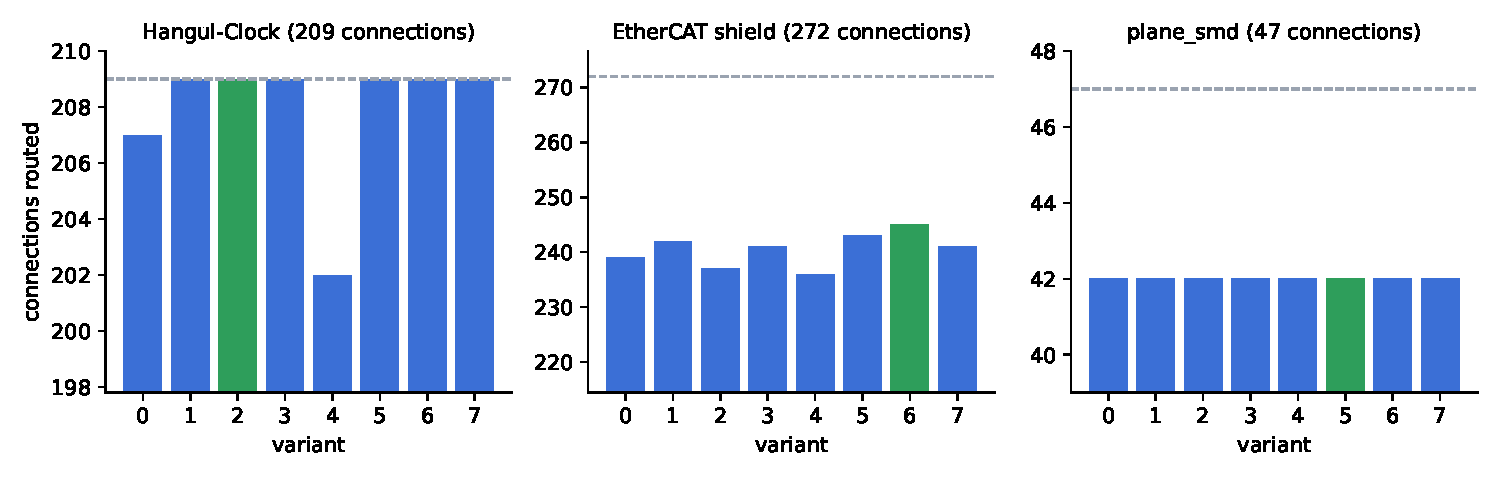
\includegraphics[width=\textwidth]{chart_variants.pdf}
\caption{Connections each variant routed in the plain portfolio (green: kept). No variant wins everywhere: variant 2 on Hangul-Clock,
6 on EtherCAT, 5 on \texttt{plane\_smd}. On Hangul-Clock five variants complete and the tie is broken by vias, then copper length;
on \texttt{plane\_smd} all eight stop at 42. That spread is why the default is a portfolio.}
\label{fig:variants}
\end{figure}

\subsection{One variant: lattice, plan and order (S15--S17)}

\step{S15 Obstacles and pitch.} Each variant builds its obstacle model (fixed copper, zone fills, keep-outs, the rule engine) and a
routing lattice. The pitch is the smallest track width plus clearance over the net classes, divided by six, rounded down to 5~$\mu$m and
held between 25 and 100~$\mu$m:
\[ p = \operatorname{clamp}\!\left(\left\lfloor \tfrac{\min_c (w_c + s_c)}{6 \cdot 5\,\mu\text{m}} \right\rfloor \cdot 5\,\mu\text{m},\; 25\,\mu\text{m},\; 100\,\mu\text{m}\right). \]
Hangul-Clock and EtherCAT get 75~$\mu$m, \texttt{plane\_smd} 25~$\mu$m. \opt{--pitch-um} sets it. The lattice is only where the
search looks: every path is turned into tracks and checked exactly before it is committed.

\step{S16 The connection plan.} Pads already joined by copper are grouped (union-find), and each net's groups are joined by a minimum
spanning tree. The edge length is the \emph{copper gap} between pads, plus a tiny share of the centre distance to break ties
(\opt{--plan-gap}, on). A pad may connect into a zone of its net through a via. The order is shortest first (variants 1, 2 and 4
change it), then the knowledge base's earlier failures move to the front, then critical nets and first nets, then buses.

\step{S17 Escape planning.} Global routing is \emph{off} by default. Variants 3 and 6 reserve escape corridors for the pins of dense
packages (at least 8 pads at 1.3 mm pitch or less): the reserved cells are closed to other nets in strict searches and cost 2 mm in
negotiated ones. On a breakout board the variant also turns on transactions (a negotiated route is kept only if the nets it ripped can
be routed again) and penalties for running along the package's pad layer.

\begin{figure}[H]
\centering
\begin{subfigure}{0.49\textwidth}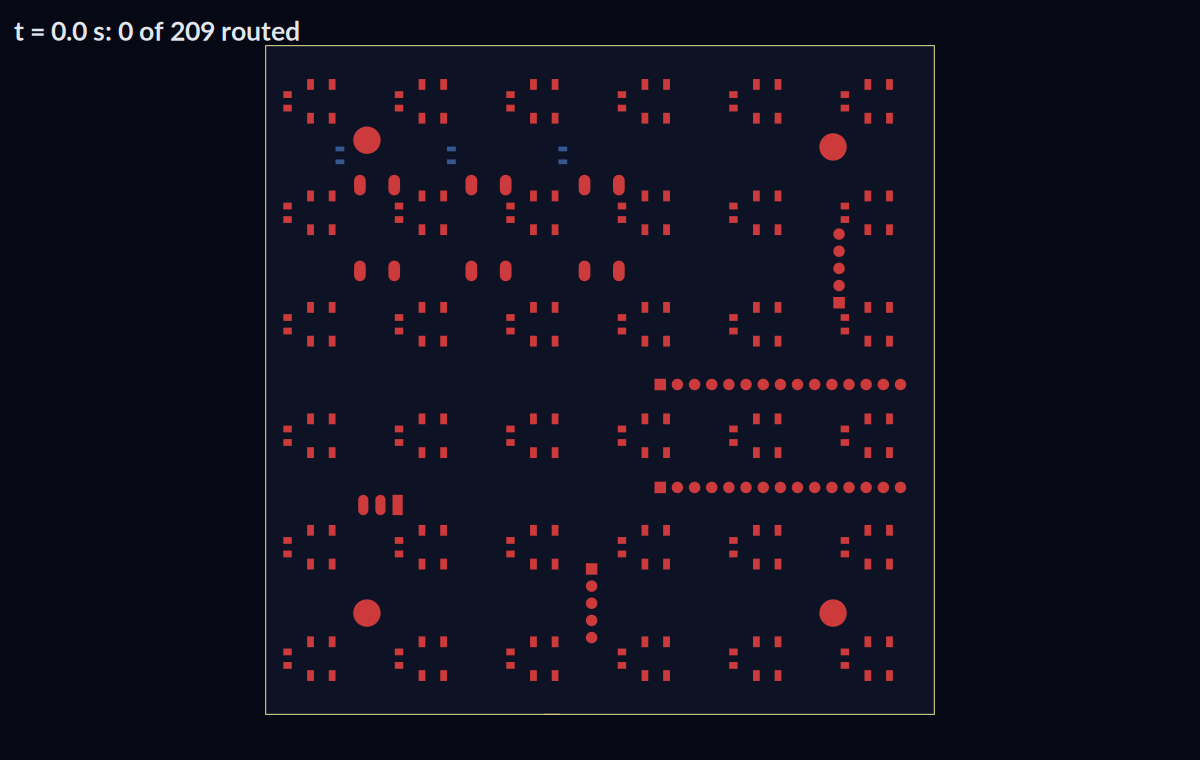
\includegraphics[width=\linewidth]{hangul_stage_0.png}\caption{start: pads and ratsnest}\end{subfigure}\hfill
\begin{subfigure}{0.49\textwidth}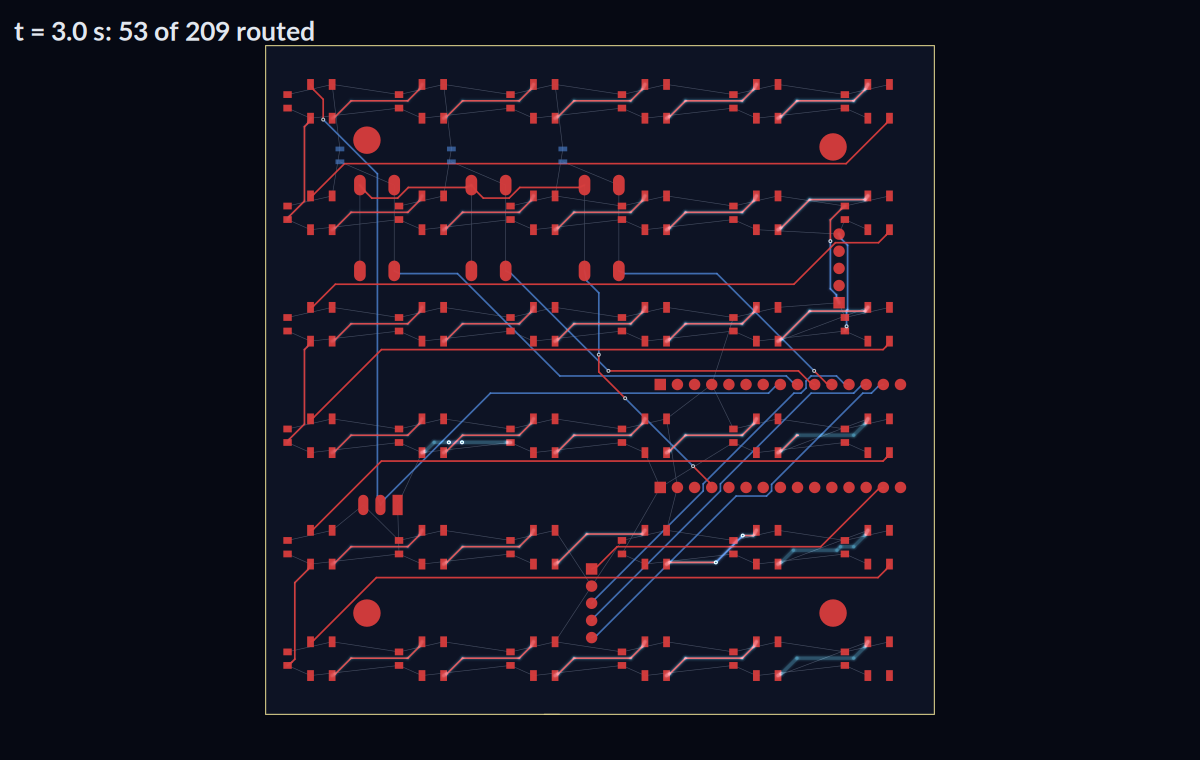
\includegraphics[width=\linewidth]{hangul_stage_1.png}\caption{a quarter routed: short connections first}\end{subfigure}\\[4pt]
\begin{subfigure}{0.49\textwidth}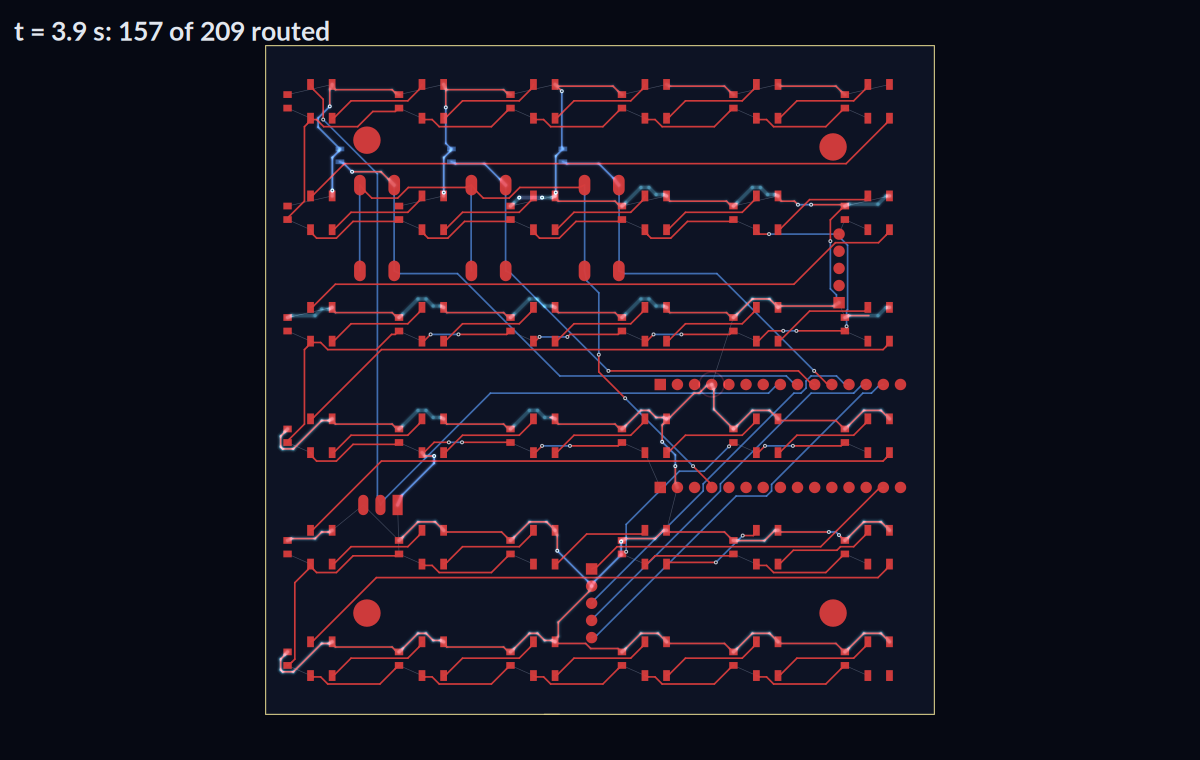
\includegraphics[width=\linewidth]{hangul_stage_2.png}\caption{three quarters: the long ones}\end{subfigure}\hfill
\begin{subfigure}{0.49\textwidth}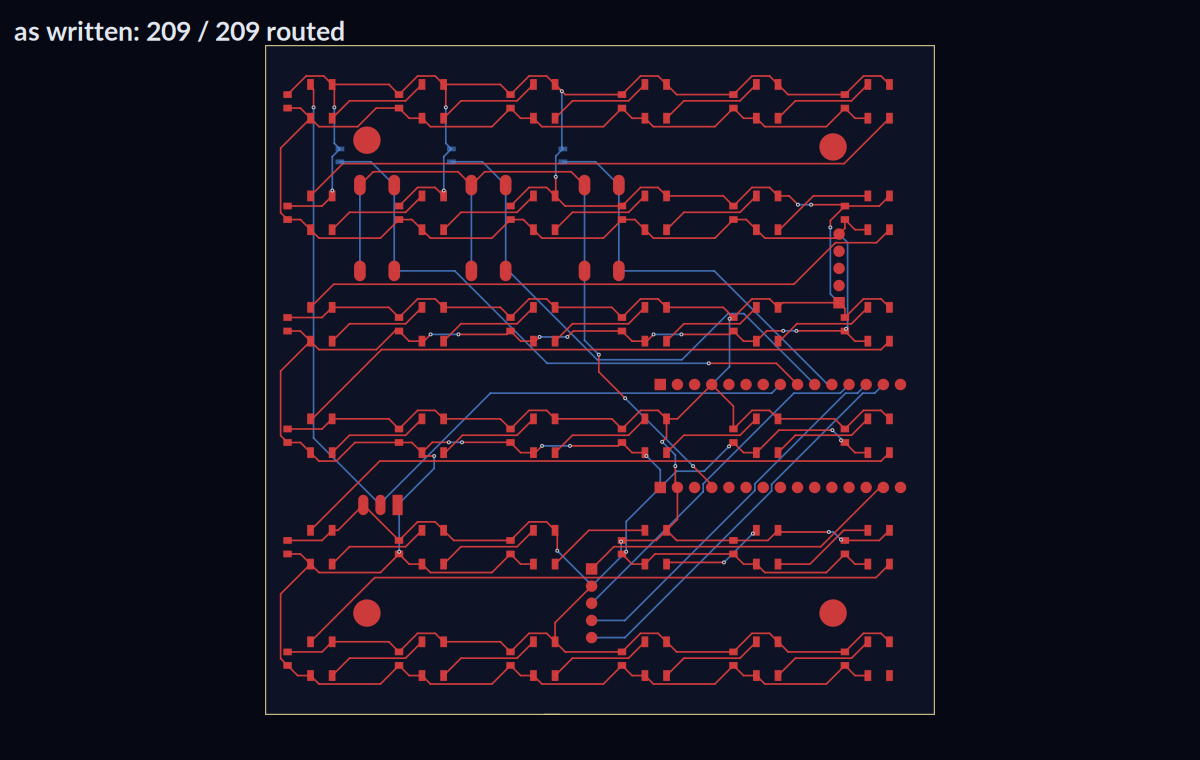
\includegraphics[width=\linewidth]{hangul_stage_3.png}\caption{as written, after clean-up}\end{subfigure}
\caption{The winning variant on Hangul-Clock, from its recorded events (\opt{--record} keeps the winner's stream). Red: top copper,
blue: bottom; grey lines: the ratsnest still to route. This variant orders longest first, so the long bus connections across the
board come early; the short pad-to-pad links fill in around them.}
\label{fig:stages}
\end{figure}

\subsection{One connection: search, check, escalate (S18)}
\label{sec:search}

Each connection is routed by an A* search on the lattice, in 8 directions on every copper layer, with vias between layers. The costs
are integers (rule 2: determinism):

\begin{figure}[H]
\centering
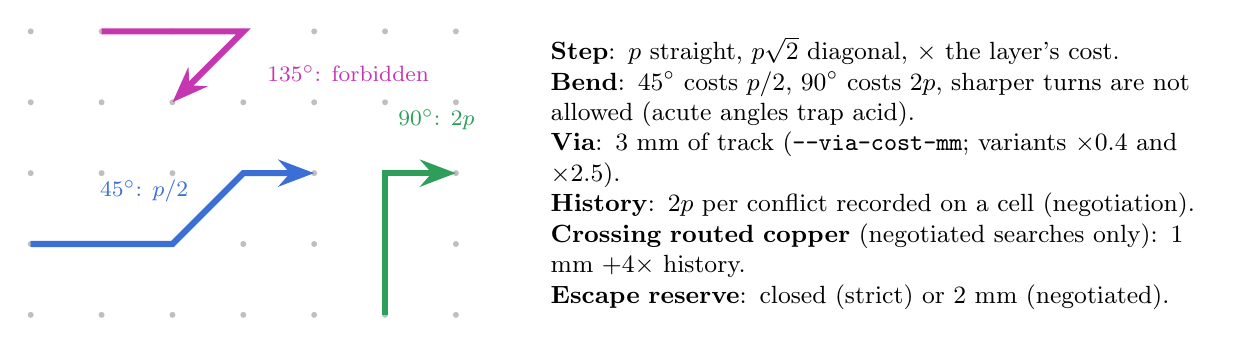
\begin{tikzpicture}[scale=0.9, font=\small]
\foreach \x in {0,...,6} \foreach \y in {0,...,4} \fill[black!25] (\x,\y) circle (1.2pt);
\draw[line width=2.2pt, accent, -{Stealth}] (0,1) -- (2,1) -- (3,2) -- (4,2);
\node[accent] at (1.6,1.75) {\footnotesize 45$^\circ$: $p/2$};
\draw[line width=2.2pt, okgreen, -{Stealth}] (5,0) -- (5,2) -- (6,2);
\node[right, okgreen] at (5.05,2.75) {\footnotesize 90$^\circ$: $2p$};
\draw[line width=2.2pt, mag, -{Stealth}] (1,4) -- (3,4) -- (2,3);
\node[mag, anchor=west] at (3.2,3.4) {\footnotesize 135$^\circ$: forbidden};
\node[align=left, anchor=west, text width=8.2cm] at (7.2,2) {
\textbf{Step}: $p$ straight, $p\sqrt2$ diagonal, $\times$ the layer's cost.\\
\textbf{Bend}: 45$^\circ$ costs $p/2$, 90$^\circ$ costs $2p$, sharper turns are not allowed (acute angles trap acid).\\
\textbf{Via}: 3 mm of track (\opt{--via-cost-mm}; variants $\times 0.4$ and $\times 2.5$).\\
\textbf{History}: $2p$ per conflict recorded on a cell (negotiation).\\
\textbf{Crossing routed copper} (negotiated searches only): 1 mm $+ 4 \times$ history.\\
\textbf{Escape reserve}: closed (strict) or 2 mm (negotiated).};
\end{tikzpicture}
\caption{The search's costs ($p$ = pitch). The heuristic is a \emph{cost-to-go field}, an exact distance map over the window computed
before the search, when the window has at least 60,000 cells; otherwise the octile distance. Fields of 500,000 cells and more are
computed on the GPU, smaller ones on the CPU; both give identical numbers (rule 3).}
\label{fig:costs}
\end{figure}

A connection climbs a ladder of rungs until one routes it (Figure~\ref{fig:tree-connection}, Table~\ref{tab:ladder}). The first search
is \emph{strict}: it may not cross other nets' copper. It looks in growing windows around the connection's bounding box: margins of 2
and 6 mm in the first pass, then 20 mm and the whole board. Each found path is turned into track segments and vias and checked
exactly against every obstacle and rule before it is committed. If the pin is boxed in, or the exact check refuses the path, forced
escapes and narrower neck-down widths are tried. From the second pass on, a \emph{negotiated} search may cross other nets' copper at a
cost; committing it rips the copper it crosses, and those connections go back into the queue (PathFinder-style negotiated congestion,
with a history cost on contested cells).

\begin{table}[H]
\centering\small
\begin{tabular}{@{}llp{9.5cm}@{}}
\toprule
Rung & When & What it tries \\
\midrule
L0 & always first & already joined by copper (e.g. through a plane via): counted as routed \\
L1, L2 & pairs, buses & coupled pair, bus lane (only with \opt{--diff-pairs}, \opt{--bus}) \\
L3 & \opt{--power-width} & strict search at the wide power width first \\
L4 & always & strict search in windows of 2, 6 (pass 0), then 20 mm and the whole board; reachability flood before a likely failure; a two-sided proof after 100,000 expansions; exact check before commit \\
L5 & boxed in or refused & forced off-lattice pad escapes, then neck-down width and a smaller via \\
L5b--L6 & options & via shove, pin rescue, via retry (\opt{--via-shove}, \opt{--rescue-in-loop}, \opt{--via-retry}; all off) \\
L7 & pass $>$ 0 & negotiated search; may rip other nets (transactional on breakout boards) \\
L8 & negotiation boxed in & negotiated escapes and neck-down; still boxed in: \emph{dead}, given up \\
L9 & \opt{--plane-informed} & join a nearby pad already on the plane (off) \\
--- & otherwise & failed: next pass, the most-failed connections first \\
\bottomrule
\end{tabular}
\caption{The per-connection ladder as implemented (\code{router.cpp:6999-7103}). Around it: up to 40 passes over the failed
connections, then up to 6 restarts that rip everything and route the hardest first (history and failure memory kept), then up to 40
diversified restarts. The result of a variant is its best state, not its last.}
\label{tab:ladder}
\end{table}

\begin{figure}[H]
\centering
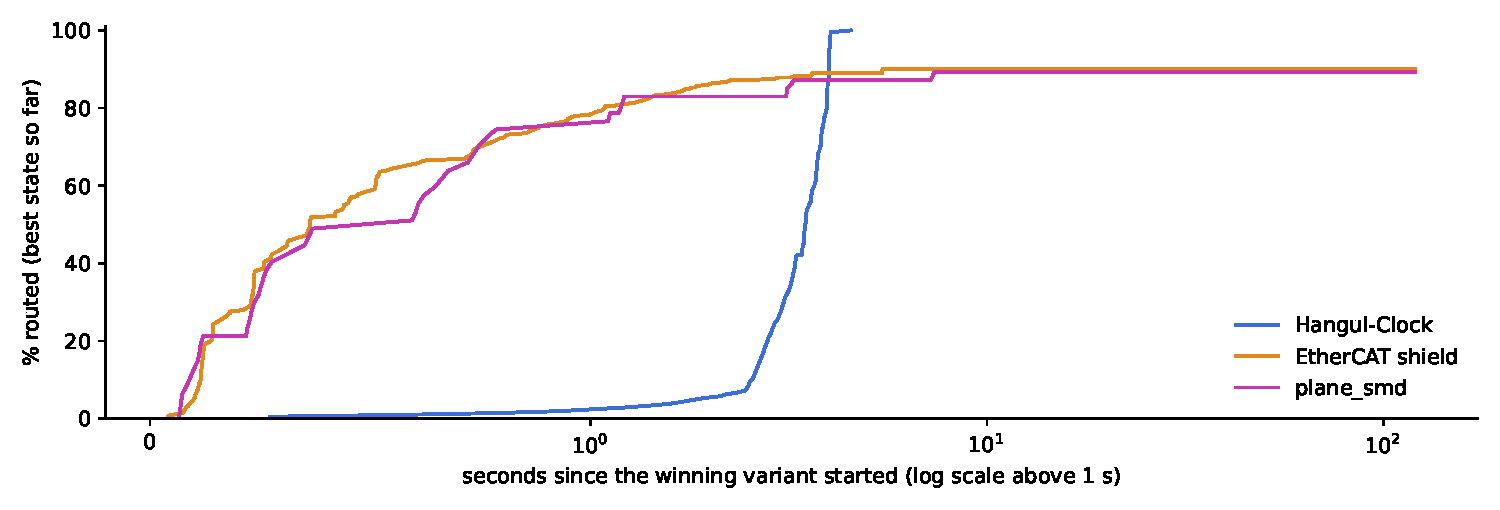
\includegraphics[width=0.92\textwidth]{chart_progress.pdf}
\caption{Connections routed over time in each run's winning variant: the best state so far, from the recorded \texttt{stats} events (a restart rips everything, but the variant returns its best state). Most connections go in the
first seconds; the rest of the time is spent on the last few, in passes and restarts. EtherCAT's winner is the fresh rescue's
portfolio, whose relaxed rounds started from scratch.}
\label{fig:progress}
\end{figure}

\begin{figure}[H]
\centering
\begin{subfigure}{0.49\textwidth}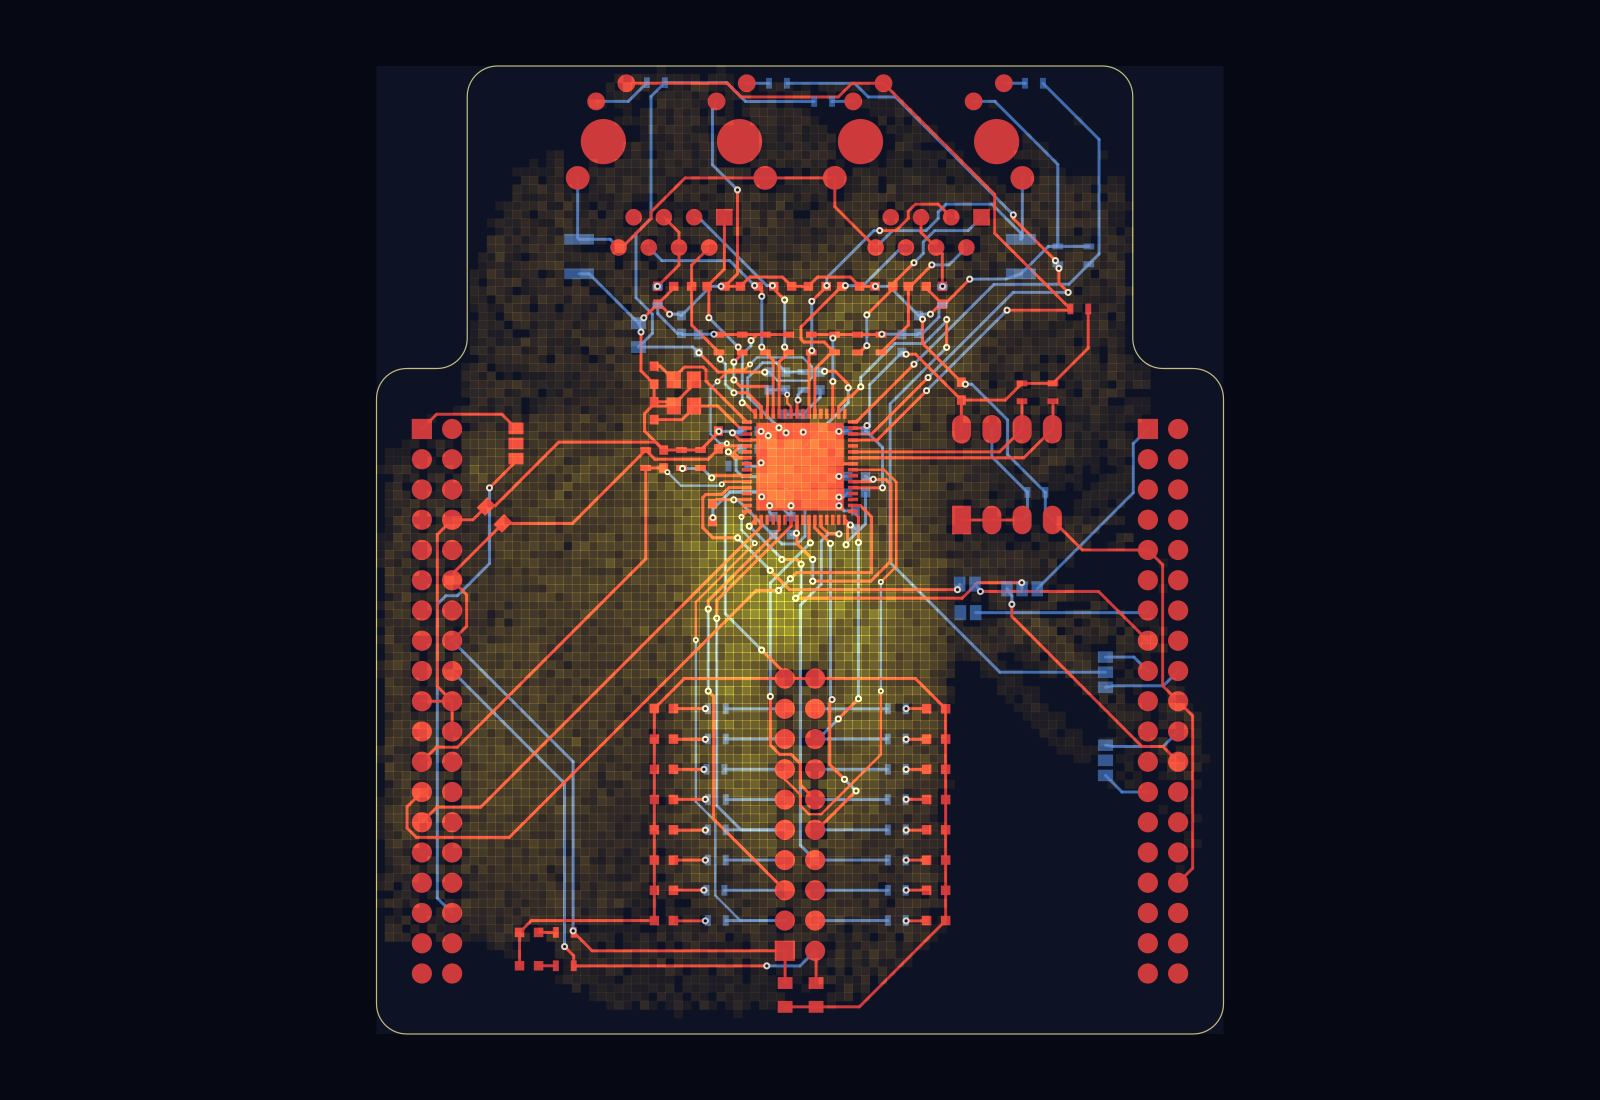
\includegraphics[width=\linewidth]{ethercat_heat.png}\caption{search effort (recorded heat map)}\end{subfigure}\hfill
\begin{subfigure}{0.49\textwidth}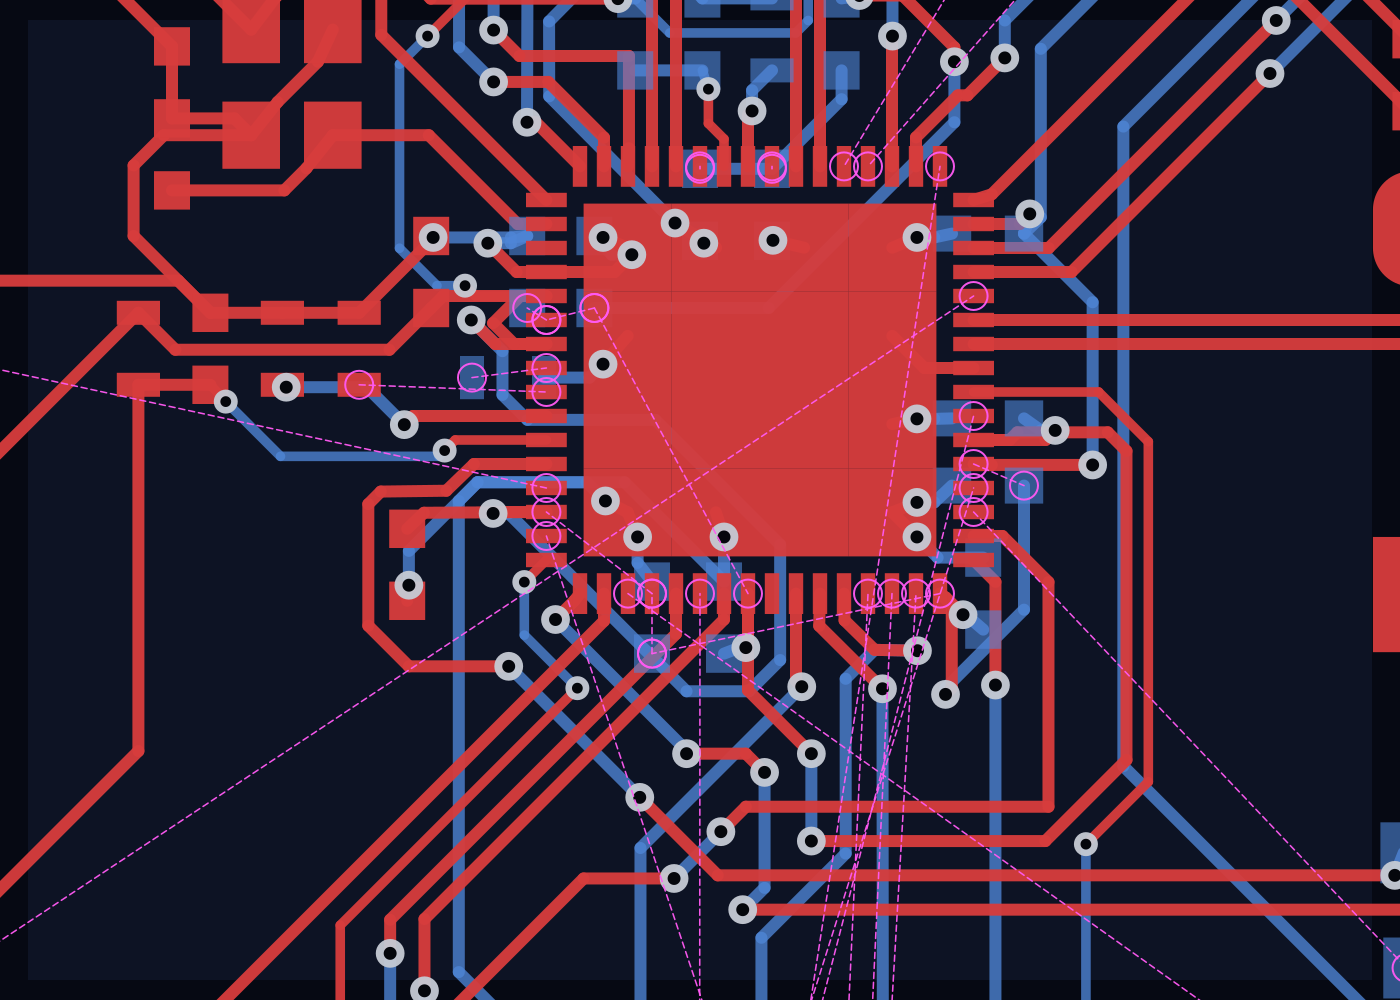
\includegraphics[width=\linewidth]{ethercat_zoom.png}\caption{round the QFN: the 25 open connections (magenta)}\end{subfigure}
\caption{EtherCAT shield. (a) The heat map the router records of where its searches expanded: almost all of the effort goes into the
QFN in the middle and the header rows below it. (b) The open connections all run into that package; the why-open proof finds all 46 of
their pins open through congestion, none walled in, so more search or more layers could finish them.}
\label{fig:ethercat}
\end{figure}

\subsection{Clean-up (S20)}

When a variant ends in its best state, it cleans up: each connection is re-routed with vias ten times dearer and kept if it is cheaper
(up to 4 rounds), a large-neighbourhood search over vias, smoothing with octilinear shortcuts (each exactly checked), and length and
skew tuning for nets with custom length rules. If the variant ended away from its best state, the best snapshot is returned \emph{without}
clean-up, unless the board has length rules (N27). On EtherCAT the logs report 172--276 connections improved per variant.

\subsection{The relax rescue (S21)}
\label{sec:rescue}

If connections are open after the plain portfolio, the run tries again with \emph{relax}: a portfolio of eight that routes under 60\,\%
and then 80\,\% of the board's clearance, moves the copper off the lattice until it meets the real rules (the legaliser), keeps the
largest conflict-free subset, and repeats, in rounds of 20 M expansions until the board is complete, 200 rounds are done, or the time is
up. A final round under the real rules keeps only legal routes. The \emph{warm} pass starts from the plain run's routes; the \emph{fresh}
pass, run only if connections are still open, starts from nothing. Each is kept only if it routes more.

\begin{figure}[H]
\centering
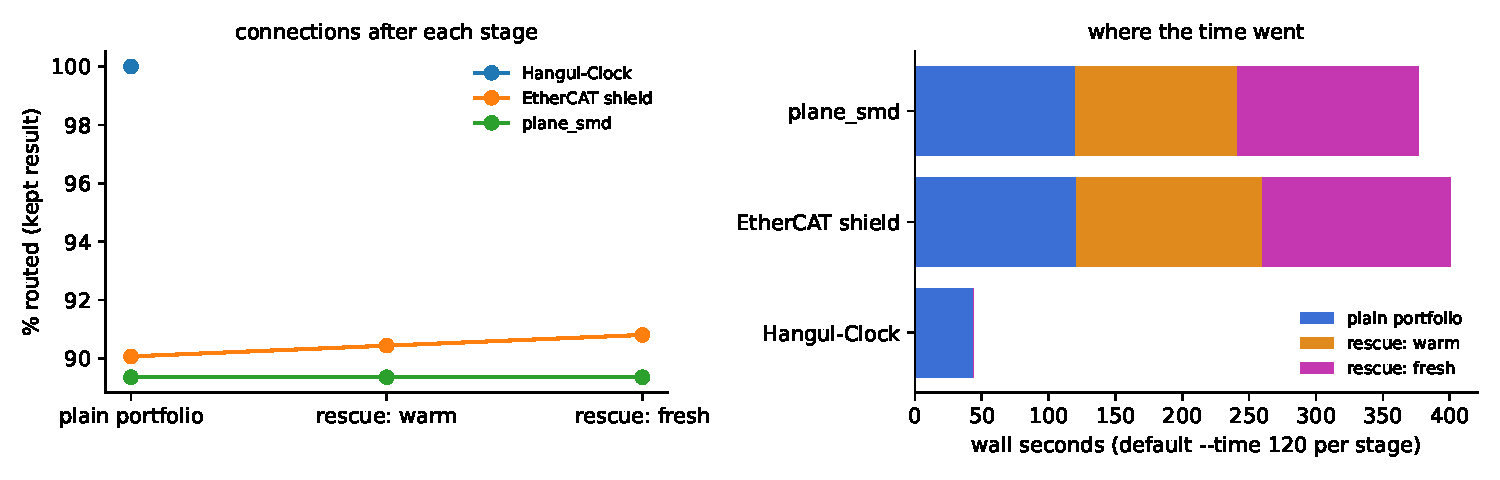
\includegraphics[width=\textwidth]{chart_ladder.pdf}
\caption{Left: the kept result after each stage. On EtherCAT the plain portfolio routed 245, the warm rescue 246, the fresh rescue 247;
on \texttt{plane\_smd} neither rescue gained, so the plain result stands. Hangul-Clock completed in the plain run and skipped the
rescue. Right: the cost. Each rescue pass has its own 120 s, so an incomplete board takes about three times \opt{--time}.}
\label{fig:ladder}
\end{figure}

\subsection{Repair, refill and the after-route passes (S22--S25)}

\step{S22} The advisor (\opt{--advisor}) is off; the knowledge base records the run. \step{S23 Repair windows} (\opt{--repair auto})
run only when the input had unlocked copper and connections are open: unlocked copper within 1, 2 and 4 mm of an open connection is
lifted and the area routed again, kept only if fewer stay open. \step{S24 Soft zones}: if the run used soft zones, the zones are
refilled for the new copper, items left unconnected are routed again on the refilled board, and thermal reliefs the new copper starved
are repaired pad by pad. \step{S25} The after-route passes (octilinear doglegs, widening power, stitching vias) are all off, except
narrowing nets to their tuning profile's widths when the project has profiles. Each is a transaction judged by connectivity and kept
only if no net gets worse.

\subsection{Writing the board (S26) and explaining the result (S27--S28)}
\label{sec:whyopen}

Only the new tracks and vias are added to the document; every other byte of the input is written back unchanged (rule 8, checked by
\texttt{tracemaker check-roundtrip}). Existing zone fills are not refilled; KiCad does that. On a board with a plane, the critical nets
found in S11 are audited: vias, length, crossings of plane voids and layer changes without a nearby return stitch.

For every pin of an open connection (up to 400) the \emph{why-open proof} floods the free space round the pin for a track of the net's
width, against the fixed copper only. A pin that no track or via can leave is \emph{walled in}: no router can connect it as placed. A pin
that only a narrower track could leave needs a neck-down; one walled in only by zone fills needs \opt{--soft-zones}; the rest are
\emph{open through congestion}: the copper routed so far is in the way, and more search or more layers can help. The log ends with
\texttt{next:} suggestions built from these classes.

\begin{figure}[H]
\centering
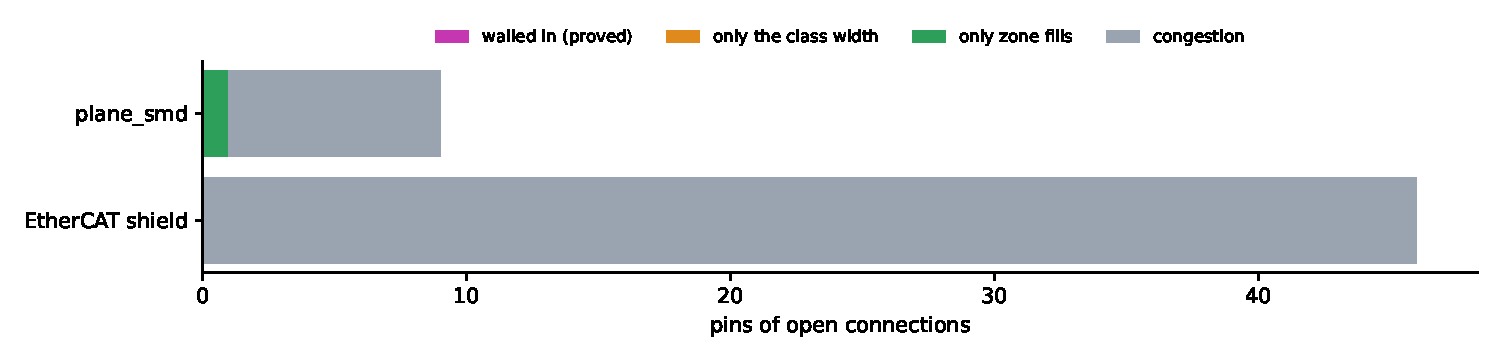
\includegraphics[width=0.92\textwidth]{chart_why_open.pdf}
\caption{The why-open proof on the two incomplete boards. EtherCAT: all 46 pins congested. \texttt{plane\_smd}: 8 congested and 1
walled in only by zone fills, for which the run suggested \opt{--soft-zones} (Section~\ref{sec:softzones}).}
\label{fig:whyopen}
\end{figure}

\begin{figure}[H]
\centering
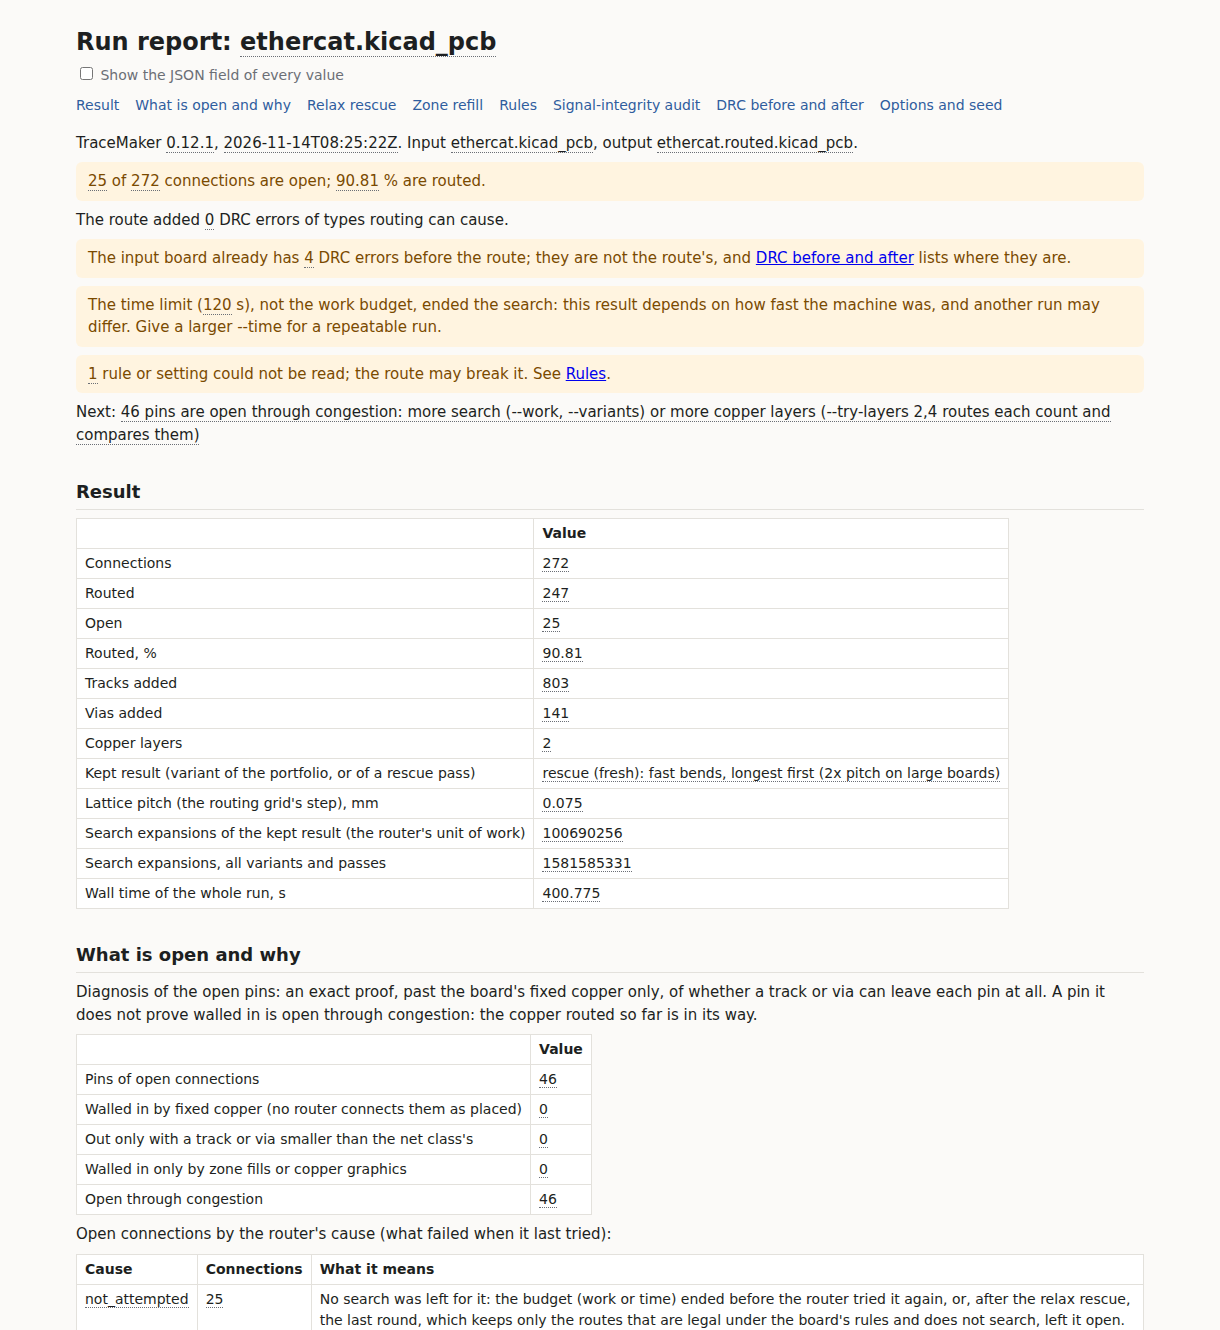
\includegraphics[width=0.82\textwidth]{report_ethercat_top.png}
\caption{The top of EtherCAT's run report (\opt{--report ethercat.html}): the result, the warning that the time limit ended the search,
the next step, and the open pins by cause and by part. Every number in the report is a field of the run's JSON.}
\label{fig:report}
\end{figure}

\step{Exit code.} 0 when every connection is routed (with soft zones: when nothing is unconnected after the refill), otherwise 3.

%% ======================================================================
\section{Options that change the default}
\label{sec:options}

\subsection{Budget and repeatability: \opt{--work}}

\begin{figure}[H]
\centering
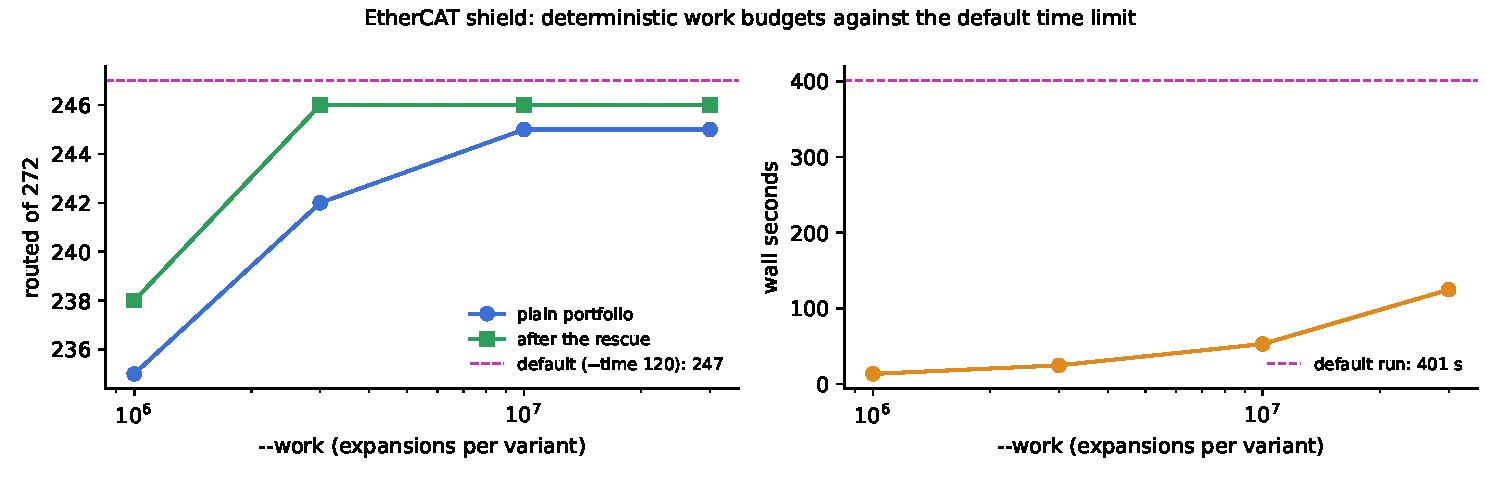
\includegraphics[width=\textwidth]{chart_budget.pdf}
\caption{EtherCAT routed with \opt{--work N --no-kb} at four budgets (each variant gets $N$ expansions; the rescue gets rounds of the
same total). At 10 M work the run routes 246 of 272 in 53 s, against 247 in 401 s for the default time-limited run, and the result is
the same on any machine and any number of threads. More work beyond 10 M changed nothing here.}
\label{fig:budget}
\end{figure}

\begin{caveat}
A default run's result depends on the machine's speed and load: its stopping rule is wall time. For results you can reproduce or
compare, pass \opt{--work} (the benchmarks use 3--10 M) and \opt{--no-kb}. \opt{--time} then only stops a run that would take too long.
\end{caveat}

\subsection{Zones as walls or as soft copper: \opt{--soft-zones}}
\label{sec:softzones}

\begin{figure}[H]
\centering
\begin{subfigure}{0.49\textwidth}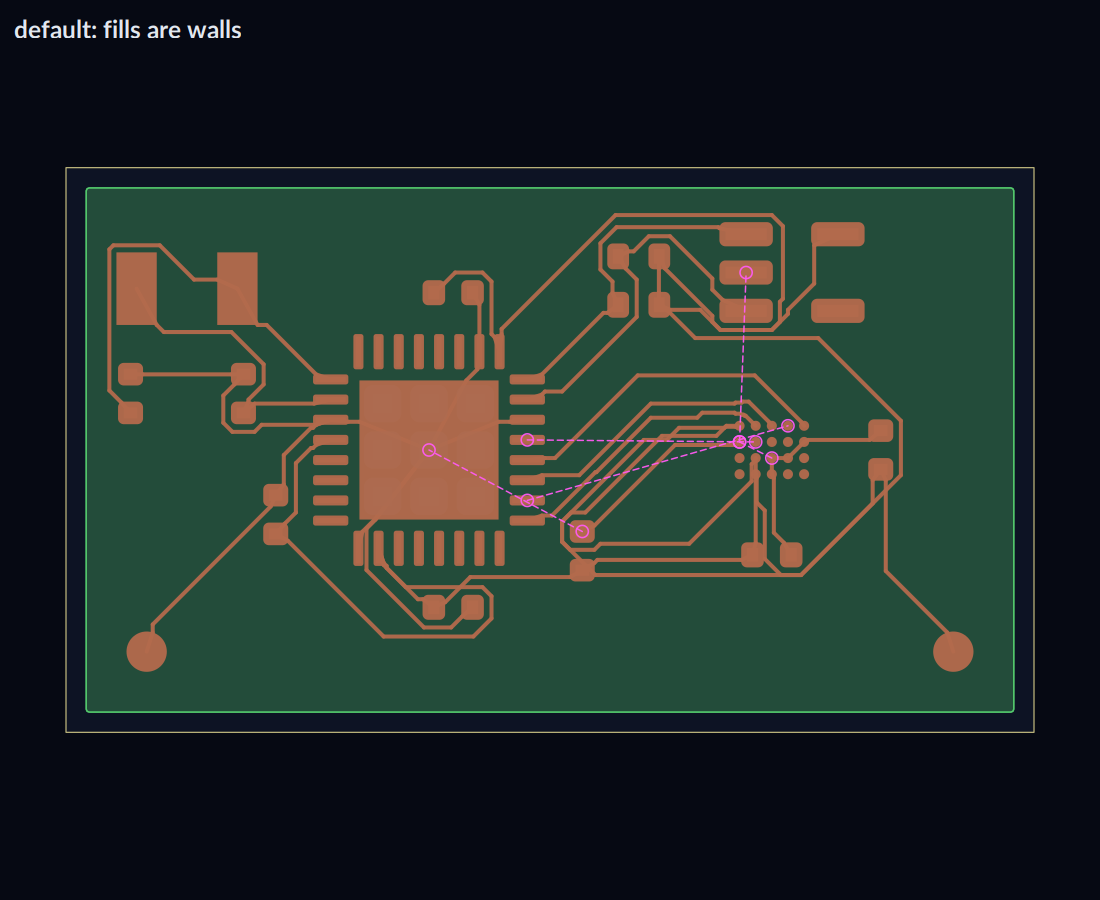
\includegraphics[width=\linewidth]{plane_default.png}\caption{default: 42 of 47}\end{subfigure}\hfill
\begin{subfigure}{0.49\textwidth}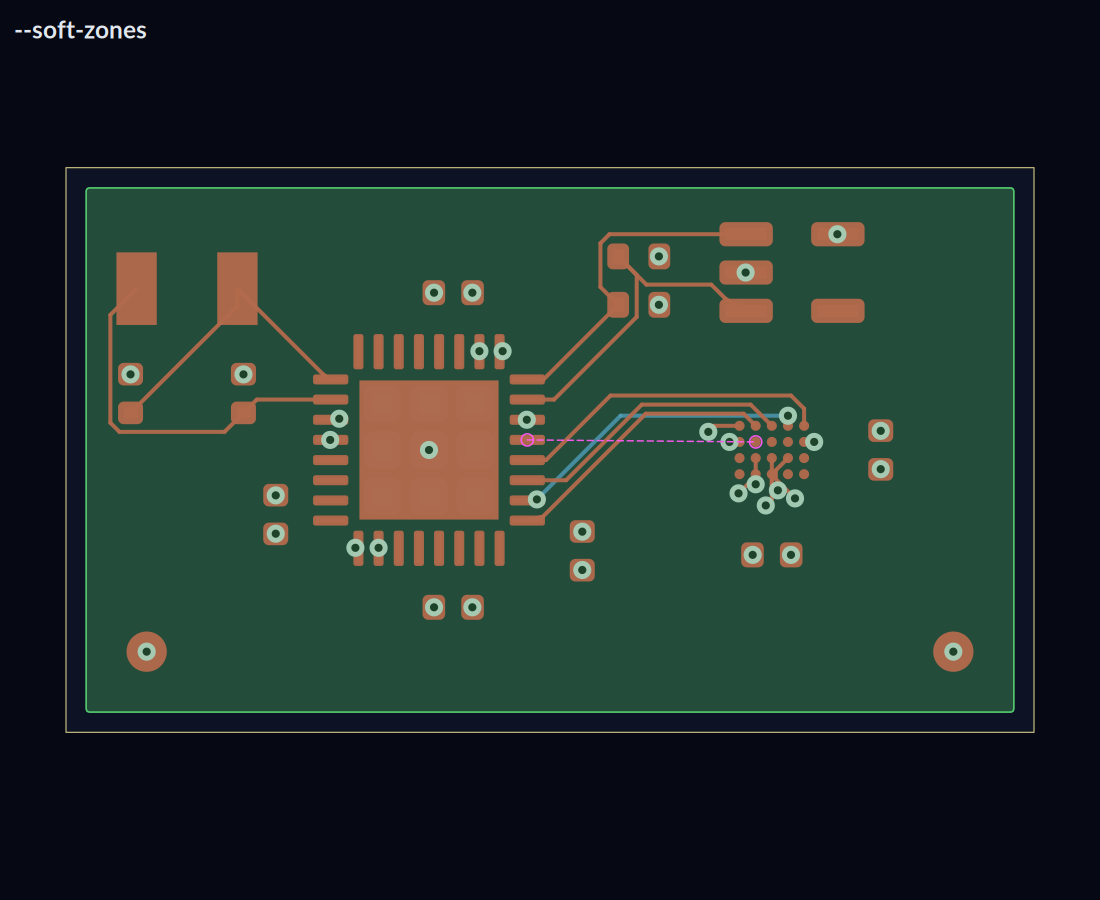
\includegraphics[width=\linewidth]{plane_soft.png}\caption{\opt{--soft-zones}: 48 of 49}\end{subfigure}
\caption{\texttt{plane\_smd} (four layers, zones in green). With the fills saved in the file they are walls, and one pin is walled in
by them alone. \opt{--soft-zones} lets other nets route through the fills, then refills the zones and routes what the refill left
unconnected. The connection plan changes with soft zones (49 connections instead of 47), so compare the open ones: 5 $\to$ 1.
The pin left over is walled in for its class's track and via, but the proof finds that a 0.25 mm via fits: a narrower class would
finish it. The refill repair was skipped because the time limit was used up, and the run read the 5 failures the default run had just
recorded in the knowledge base.}
\label{fig:soft}
\end{figure}

\subsection{Finished-looking copper: \opt{--power-width} and \opt{--octilinear}}

\begin{figure}[H]
\centering
\begin{subfigure}{0.32\textwidth}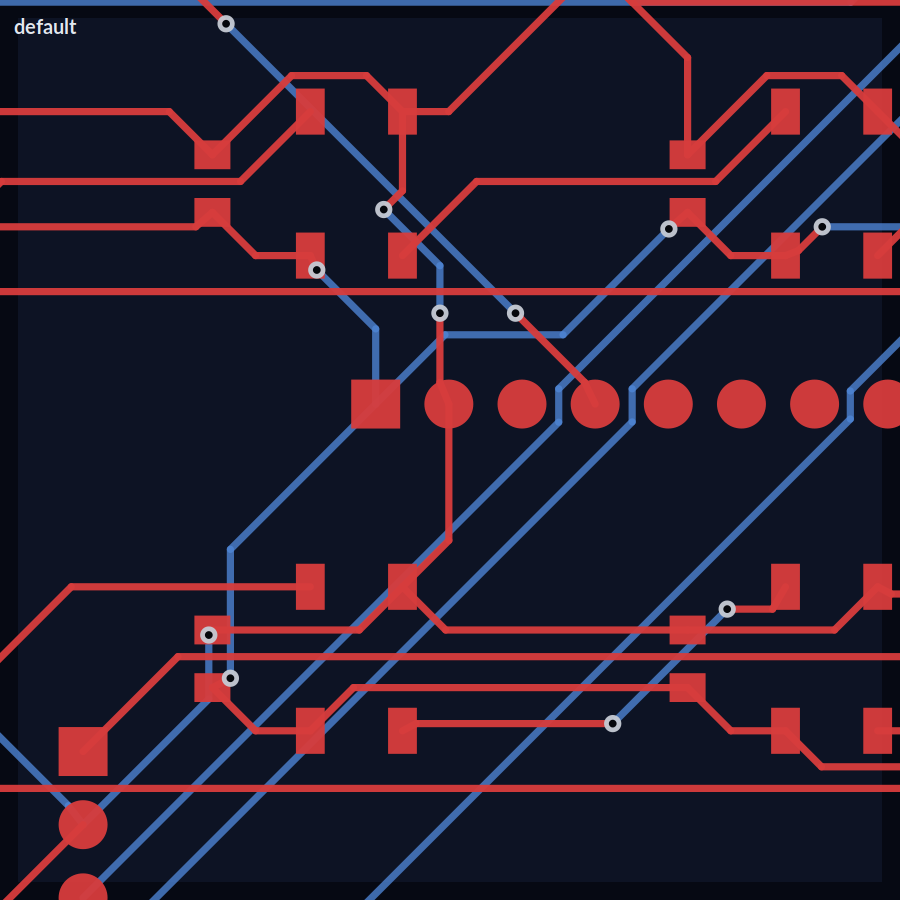
\includegraphics[width=\linewidth]{opt_plain.png}\caption{default}\end{subfigure}\hfill
\begin{subfigure}{0.32\textwidth}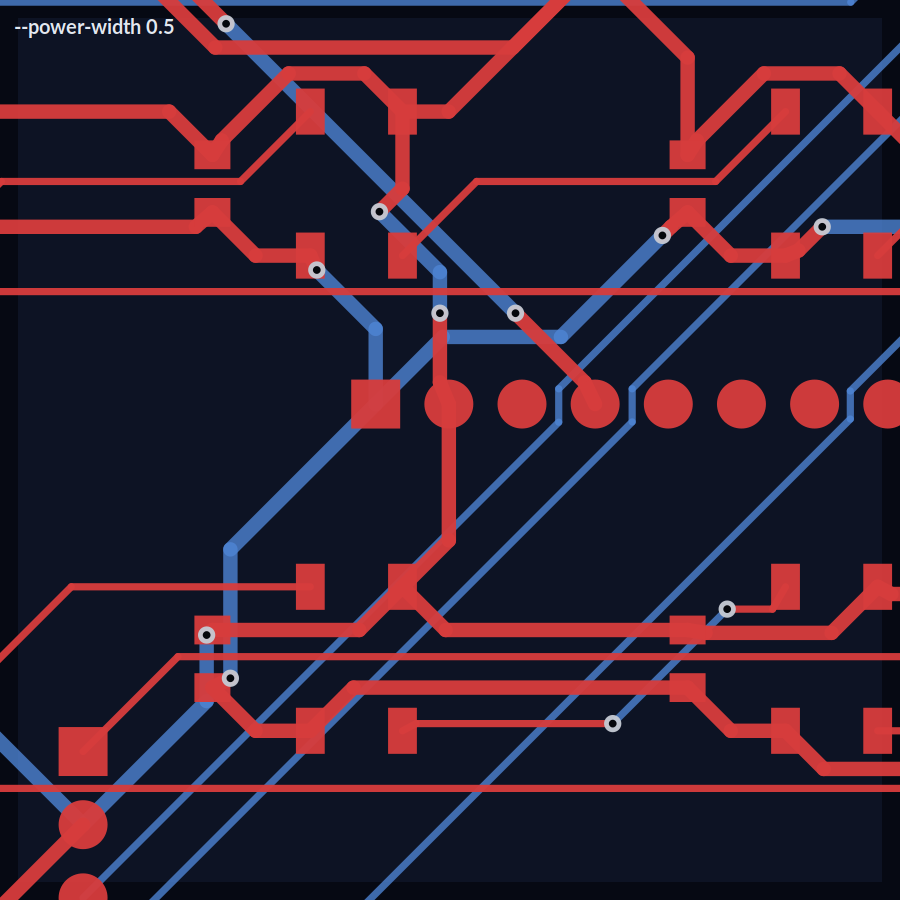
\includegraphics[width=\linewidth]{opt_pw.png}\caption{\opt{--power-width 0.5}}\end{subfigure}\hfill
\begin{subfigure}{0.32\textwidth}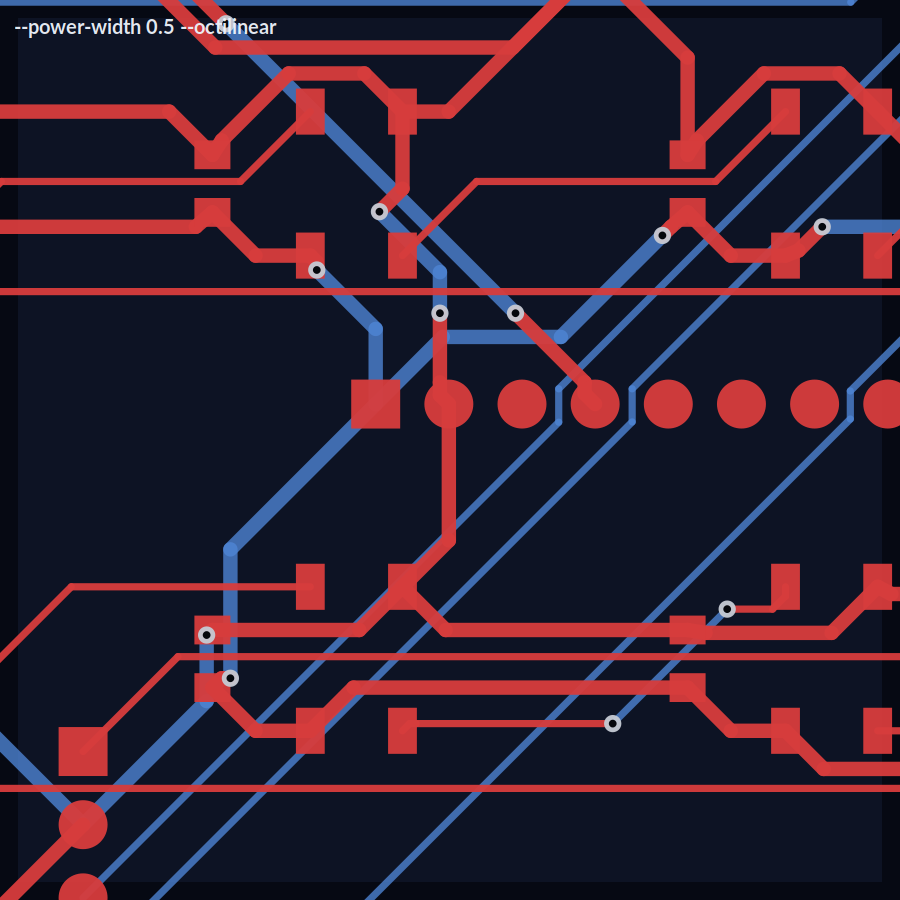
\includegraphics[width=\linewidth]{opt_m23.png}\caption{\opt{+ --octilinear}}\end{subfigure}
\caption{A 30 $\times$ 30 mm corner of Hangul-Clock at 3 M work, same seed. \opt{--power-width 0.5} routes supply nets at 0.5 mm from
the start (supply copper at $\geq$ 0.5 mm: 0\,\% $\to$ 100\,\% on this board, D184); \opt{--octilinear} replaces off-angle segments
by 0/45/90$^\circ$ doglegs where the exact check allows (84 $\to$ 60 here, $-39$\,\% over 80 benchmark boards, D187). Both are off
in the command-line default and on in the KiCad plugin.}
\label{fig:style}
\end{figure}

\subsection{The options, grouped}

\small
\begin{longtable}{@{}p{4.3cm}p{2.5cm}p{8.4cm}@{}}
\toprule
Option & Default & Effect \\
\midrule
\endhead
\multicolumn{3}{@{}l}{\textbf{Budget and time}}\\
\opt{--time S} & 120 & wall-clock limit per variant from its own start, and again per later stage \\
\opt{--work N} & none & deterministic budget: expansions per variant (each gets all of it); output independent of threads and machine \\
\opt{--time-total T} & none & one deadline for the whole job; the plain run gets $0.75\,T$ \\
\opt{--max-passes}, \opt{--max-restarts} & 40, 6 & passes over failed connections; planned restarts (+40 diversified) \\
\multicolumn{3}{@{}l}{\textbf{Portfolio}}\\
\opt{--threads N} & 8 & worker threads; also the portfolio size without \opt{--work} (at most 8) \\
\opt{--variants N} & auto (8) & portfolio size; above 8 adds seeded variants (up to 64) \\
\opt{--halving} & off & successive halving when variants exceed threads \\
\opt{--seed} & 1 & base seed of every variant \\
\opt{--kb FILE}, \opt{--no-kb} & on & failure memory: earlier failures first; recorded after the run \\
\multicolumn{3}{@{}l}{\textbf{Search and costs}}\\
\opt{--pitch-um} & auto & lattice pitch; auto = $\min(w + s)/6$, 25--100 $\mu$m \\
\opt{--via-cost-mm} & 3.0 & via cost as track length \\
\opt{--heuristic-weight} & 1.0 & weighted A* ($>1$: faster, not optimal) \\
\opt{--no-rip-up} & rip-up on & no negotiation \\
\opt{--fast-bends} & mixed & one state per lattice point in every variant \\
\opt{--no-field}, \opt{--no-gpu} & on, auto & octile heuristic only; CPU fields (same result) \\
\opt{--global} & off & global routing corridors first \\
\opt{--crowded-source} & 4 of 8 & every strict search from the crowded end \\
\opt{--micro-vias}, \opt{--blind-vias} & off & allow those via types where the board does \\
\opt{--layer-dir-pen}, \opt{--layer-dir} & auto & cost of steps against a layer's preferred direction (0.3 on breakouts) \\
\multicolumn{3}{@{}l}{\textbf{Dense packages}}\\
\opt{--escape-plan} & 2 of 8 & escape corridors in every variant \\
\opt{--escape-flow} & off & min-cost-flow escapes for deep BGAs \\
\opt{--via-in-pad} & off & vias in pads for inner balls \\
\multicolumn{3}{@{}l}{\textbf{Rescue and repair}}\\
\opt{--no-rescue} & rescue on & skip the relax rescue \\
\opt{--rescue-mode} & both & warm, fresh or both \\
\opt{--relax} & off & relax from the start (then no rescue) \\
\opt{--repair auto|on|off} & auto & repair windows (auto: only if the input had unlocked copper) \\
\opt{--endgame}, \opt{--rescue R}, \opt{--via-shove}, \opt{--via-retry} & off & last-connection tools of M22 (measured, not adopted, D179) \\
\opt{--advisor CMD} & none & an external advisor consulted when connections stay open \\
\multicolumn{3}{@{}l}{\textbf{Clean-up and style}}\\
\opt{--no-optimize} & clean-up on & skip via saving, smoothing and length tuning \\
\opt{--octilinear} & off & 0/45/90$^\circ$ doglegs for off-angle segments \\
\multicolumn{3}{@{}l}{\textbf{Power, pours and zones}}\\
\opt{--power-width MM} & off & supply nets routed wide first, necked at pads \\
\opt{--widen-power} & off & widen supply tracks after routing \\
\opt{--soft-zones} & auto & fills do not block; refill and route again afterwards \\
\opt{--no-fill-planes} & fill on & do not fill unfilled zones in memory \\
\opt{--pour auto|NET@L} & none & generate a pour \\
\opt{--stitch-vias} & none & stitching vias (planes, return paths) \\
\multicolumn{3}{@{}l}{\textbf{Rules and nets}}\\
\opt{--component-rules} & off & detected component rules: keep-outs, classes \\
\opt{--diff-pairs} & off & coupled differential pairs \\
\opt{--si-rules} & off & critical nets first, dearer vias, plane-split cost \\
\opt{--no-critical-audit} & audit on & skip the return-path audit on boards with a plane \\
\opt{--only-net}, \opt{--skip-net} & none & staged routing \\
\multicolumn{3}{@{}l}{\textbf{Output}}\\
\opt{--json}, \opt{--report} & none & summary JSON; designer's report (HTML or Markdown) \\
\opt{--no-why-open} & proof on & skip the why-open proof \\
\opt{--view}, \opt{--record} & off & live viewer; event recording (not together) \\
\opt{--try-layers 2,4} & off & route each layer count and compare \\
\bottomrule
\end{longtable}
\normalsize

%% ======================================================================
\section{Where the documents and the code disagree}
\label{sec:disagree}

The design documents are meant to be the source of truth. Reading the code for this report turned up these differences and
surprising defaults. They are listed so they can be fixed, in the code or in the documents (M25).

\begin{enumerate}
\item \textbf{The escalation ladder.} Doc 05 §6 describes rungs R0--R7. R0 (search in a global corridor) needs \opt{--global} (off), R3
  exists only as the job-level repair windows, R4 and R5 were never built, R6 is \opt{--cut-report} (off). The real ladder is
  Table~\ref{tab:ladder}.
\item \textbf{The search.} §5.2 says bidirectional A* with a radix heap; the code is a one-directional A* on a binary heap, with a
  60,000-expansion reverse probe on the first window.
\item \textbf{Parallelism.} §5.3 says connections with disjoint windows are routed in parallel; inside a variant they are routed one after
  another. Threads run portfolio variants.
\item \textbf{The cost formula.} §5.1's cost is multiplicative; the code adds integer terms (Figure~\ref{fig:costs}).
\item \textbf{The package penalty} comment (\code{router.hpp:115}) says it applies on any two-layer board with a ball-grid package;
  it applies only on breakout boards.
\item \textbf{Determinism.} A default run is limited by time and reads and writes the knowledge base, so two runs can differ.
\item \textbf{Wall time} for an incomplete board is up to about three times \opt{--time}; relax rounds check the time only at their start.
\item \textbf{The pass stall test} uses the whole run's rip count (\code{router.cpp:7156}): after any rip, a pass without gain does
  not end the passes, which then run on to 40 or the budget. Whether this is intended is not clear.
\item \textbf{Clean-up} is skipped when a variant ends away from its best state, although a comment says smoothing always runs.
\item \textbf{Unreadable rules.} Rule 6 of the project says never to route on rules that could not be read and to be conservative. A custom rule
  whose condition cannot be parsed is \emph{ignored}; only conditional hole rules are widened. A missing project file is reported only in
  \opt{--report}.
\item \textbf{Net-name clearance rules} silently turn off the cost-to-go fields (and so the GPU) in every variant.
\item \textbf{Critical-net detection} runs on every board with a plane, even with component rules off (as an audit).
\item \textbf{Rescue summary fields}: §68 names \texttt{rounds} and \texttt{round\_work}; the JSON has \texttt{routed\_before},
  \texttt{routed\_after}, \texttt{passes} and others.
\item \textbf{\opt{--escape-plan}'s help} does not say that two of the eight default variants already plan escapes.
\item \textbf{Tuning profiles} change widths and add per-layer rules with no option given.
\item \textbf{The variant count follows \opt{--threads}}: \opt{--threads 4} runs only the first four variants.
\item \textbf{Unlocked input copper} is never ripped by the router; only the repair windows can lift it.
\item \textbf{Saved fills change the run}: a board with an unfilled zone routes with soft zones, the same board saved after a refill
  routes with the fills as walls.
\item \textbf{\opt{--record} with \opt{--view}}: the recording is silently skipped (\code{route_job.cpp:403}).
\end{enumerate}

%% ======================================================================
\appendix
\section{How this report was made}

\begin{itemize}
\item \textbf{The pipeline and the decision tree} come from reading \code{src/app/main.cpp}, \code{src/app/route_job.cpp},
  \code{src/route/router.cpp} and their headers at commit \texttt{e6614af}; each node carries its source line. Doc 05 sections and the
  decision records (D47, D101, D143, D160, D163, D184, D186, D187, D188 and others) were used for names and history.
\item \textbf{The runs}: \texttt{reports/routing-report/runs/}. Default runs:
  \opt{tracemaker route B.kicad_pcb -o B.routed.kicad_pcb --record B.jsonl --report B.html --json B.json}.
  Budget runs: \opt{--work N --no-kb --time 3600 --threads 8}. Soft zones: \opt{--soft-zones}. The style comparison reuses the
  M23 video's runs (\texttt{reports/m23video}, 3 M work).
\item \textbf{The figures}: \texttt{figs.py} (boards, drawn from the recordings and the written boards in the viewer's colours),
  \texttt{charts.py} (matplotlib, from the JSON summaries and recorded \texttt{stats} events), \texttt{gen\_trees.py} (the decision
  trees), the KiCad 10.0.6 3D render, and a headless-browser screenshot of the run report.
\item \textbf{Build}: \texttt{tectonic tex/report.tex}.
\end{itemize}

\end{document}
